\documentclass[10pt,journal,onecolumn]{IEEEtran}
\usepackage[utf8]{inputenc}
\usepackage[T1]{fontenc}
\usepackage{amsmath,amssymb,amsfonts}
\usepackage{booktabs}
\usepackage{tabularx}
\usepackage{graphicx}
\usepackage{hyperref}
\usepackage[margin=0.75in]{geometry}
\begin{document}
\title{Physics-Informed Variational RBF-KAN for Data-Scarce Cyber-Physical Control: Exact Differentiable Inverse Optimization and Symbolic Kinetic Recovery in Industrial HiPCO Nanotube Synthesis}
\author{Aakshay Chordia\\ \textit{Department of Electronics and Communication Engineering, PES University, Bengaluru, India}}
\maketitle
\begin{abstract}
Industrial synthesis of single-walled carbon nanotubes (SWCNTs) by high-pressure carbon monoxide (HiPCO) disproportionation operates near $60\text{ atm}$ and $950^\circ\text{C}$, where certification-grade outcomes are resolvable only by destructive post-run spectroscopy. This imposes a dual obstruction: validated ground truth is restricted to $N = 50$ factory campaigns, of which $20$ ($40.0\%$) failed certification, and no deployed surrogate supplies the analytical gradients required for closed-loop setpoint recovery. Dense multi-layer perceptrons (MLPs) memorize noise in this regime, collapsing to mean $R^2 = 0.386$, while gradient-boosted trees furnish $\nabla_{\mathbf{u}} f = \mathbf{0}$ Lebesgue-almost-everywhere and force practitioners onto derivative-free search that consumes $3,754.0\text{ ms}$ per query at a $12.5\%$ Karush-Kuhn-Tucker (KKT) safety violation rate. We introduce the Physics-Informed Variational Radial Basis Function Kolmogorov-Arnold Network (PI-VRBF-KAN). A deterministic $167$-equation transport operator $\mathcal{P}: \mathcal{U} \subset \mathbb{R}^7 \to \mathbb{R}^{11}$ first absorbs the stiff compressible-continuity, Chapman-Enskog, and NIST-JANAF Boudouard conservation laws, distilling $110$ raw OPC-UA historian channels by $83.6\%$ into $\mathbf{x} = [\mathbf{u}, \mathbf{z}] \in \mathbb{R}^{18}$; the network therefore learns only smooth residual kinetic couplings onto $\mathbf{y} \in \mathbb{R}^9$. A correlation-preserving Gaussian copula manifold ($N_{\text{synth}} = 5,000$; Frobenius divergence $\left\|\mathbf{C}_{\text{real}} - \mathbf{C}_{\text{synth}}\right\|_F = 0.0493 \ll 0.15$) pre-trains global curvature before fold-isolated factory fine-tuning. Under $5$-fold cross-validation with all standardization, copula covariance extraction, and hyperparameter selection confined strictly within training folds, the $1,305$-parameter topology $[18 \to 16 \to 9]$ attains multi-target mean $R^2 = 0.997 \pm 0.002$—Yield $R^2 = 0.998$ ($\text{MAE} = \pm 0.03\text{ g}$), Raman $G/D$ $R^2 = 0.999$ ($\pm 0.08$), UV-Vis purity $R^2 = 0.999$ ($\pm 0.77\%$), axial Fe residue $R^2 = 0.992$ ($\pm 5.10\text{k ppm}$)—at $3.3\ \mu\text{s}$ forward latency. These residuals coincide with the analytical repeatability floor of plant instrumentation ($\pm 0.01\text{ g}$ microbalance, $\pm 5.0\%$ Raman), establishing that the model has saturated measurement precision rather than fit noise. Superiority over XGBoost is significant at $\Delta R^2 = +0.283$ ($t = 7.55$, $p = 0.00165$, Wilcoxon $p = 0.00794$, Cohen's $d = 3.38$). Exploiting the $\mathcal{C}^\infty$-analytic Gaussian edge kernels, a multi-start Augmented Lagrangian autograd solver recovers Pareto-optimal setpoints in $24.5\text{ ms}$—$153.2\times$ faster than genetic search, $63,092.4\times$ under $1,000$-query vectorization—with $0.0\%$ KKT violations ($0/1,000$) and $L_2$ tracking error $0.042$, certified engine-in-the-loop against the calibrated transport twin as the mandatory safety gate preceding live DCS write-access. Finally, $L_1$ edge pruning reduces the bipartite graph to its minimal active causal skeleton, from which BIC-penalized Levenberg-Marquardt snapping recovers closed-form rate laws with critical thresholds at $T^\textit{ = 1,042.00^\circ\text{C}$, $P_{\text{crit}} = 25.00\text{ atm}$, $Q_{\text{H2O}}^} = 18.20\text{ ppmv}$, and $Q_{\text{Fe}}^* = 220.00\text{ SLPM}$ ($R^2_{\text{sym}} \ge 0.994$), each corresponding to an independently documented Arrhenius, Langmuir-Hill, water-etching, or Ostwald-ripening mechanism.
\end{abstract}
\textbf{Keywords}: Kolmogorov-Arnold Networks (PI-VRBF-KAN); Data-Scarce Industrial Machine Learning; Single-Walled Carbon Nanotubes (SWCNTs); Boudouard Disproportionation; Gaussian Copula Bootstrapping; Augmented Lagrangian Autograd Inversion; KKT Safety Certification; Engine-in-the-Loop Validation; Symbolic Kinetic Rate Law Discovery; Cyber-Physical Manufacturing Systems.

\section{Introduction}
\subsection{Industrial Context and the Certification Bottleneck}
Single-walled carbon nanotubes (SWCNTs) underpin next-generation semiconductor channels, aerospace structural composites, and high-density energy-storage electrodes by virtue of axial tensile strength exceeding $50\text{ GPa}$, ballistic thermal transport, and tunable electronic band structure (Baughman, Zakhidov, & de Heer, 2002). Among commercial routes, High-Pressure Carbon Monoxide (HiPCO) disproportionation remains the premier continuous gas-phase technique for pristine small-diameter SWCNTs (Bronikowski, Willis, Colbert, Smith, & Smalley, 2001; Nikolaev et al., 1999). Volatile iron pentacarbonyl, $\text{Fe(CO)}_5$, pyrolyzes within a turbulent high-pressure carbon monoxide stream to nucleate sub-nanometer iron aerosol clusters, which catalyze the exothermic Boudouard equilibrium:

\begin{equation}
2\text{CO} \rightleftharpoons \text{C}_{(\text{SWCNT})} + \text{CO}_2, \qquad \Delta H^\circ = -172.5\text{ kJ/mol}.
\end{equation}
Commercial operation is bottlenecked not by reaction chemistry but by observability. Operators regulate coupled multivariable interactions near $60\text{ atm}$ and $950^\circ\text{C}$, where an uncompensated thermal excursion of $\pm 10^\circ\text{C}$ displaces gas residence time and transports the reactor across thermodynamic equilibrium boundaries. Yield maximization accelerates catalyst coalescence through Ostwald ripening, generating amorphous-carbon-encapsulated metal aggregates that depress Raman crystallinity and elevate acid-insoluble iron ash beyond $250,000\text{ ppm}$. Because these outcomes resolve only through destructive post-run Raman, UV-Vis-NIR, and inductively coupled plasma mass spectrometry (ICP-MS) assay, the plant operates open-loop over a multi-day latency. Across the audited campaign record, $20$ of $50$ batches ($40.0\%$) failed commercial certification.

\subsection{Why Conventional Surrogates Fail: Representation}
The first failure mode is representational. Deep multi-layer perceptrons (MLPs) parameterized by $7,625$ dense nodal weights distribute capacity across $O(d^2)$ hyperplane intersections in the $18$-dimensional feature space. With $N = 50$ observations, the ratio of free parameters to constraints exceeds $150 : 1$, and the optimizer interpolates analytical assay noise rather than kinetic structure. Empirically, the Deep MLP collapses to mean $5$-fold cross-validation $R^2 = 0.386 \pm 0.114$, and its degradation is worst precisely where physics is most non-linear: axial Fe residue falls to $R^2 = 0.120$.

Gradient-boosted decision-tree ensembles resist this collapse on bulk mass yield ($R^2 = 0.893$) because axis-aligned recursive partitioning imposes a strong piecewise-constant prior. However, trees train independent, uncoupled hierarchies per output channel. Lacking any shared internal representation of carbon mass balance or catalyst ripening, XGBoost degrades sharply on structurally sensitive targets, reaching only $R^2 = 0.764$ on Raman $G/D$ and $R^2 = 0.408$ on Fe residue.

\subsection{Why Conventional Surrogates Fail: Invertibility}
The second failure mode is more fundamental and forecloses closed-loop control entirely. Decision-tree ensembles partition $\mathcal{U}$ into piecewise-constant hyper-rectangles, so the forward map is locally constant and:

\begin{equation}
\nabla_{\mathbf{u}} f(\mathbf{u}) = \mathbf{0} \quad \text{for Lebesgue-almost-every } \mathbf{u} \in \mathcal{U},
\end{equation}
with the gradient undefined on the measure-zero set of split boundaries. No descent direction exists. Control engineers are therefore forced onto derivative-free metaheuristics—Genetic Algorithms (GA), Nelder-Mead simplex search, or Gaussian Process Bayesian Optimization—whose cost and safety profile are incompatible with a plant Distributed Control System (DCS) scan cycle. Single-query GA optimization consumes a mean of $3,754.0\text{ ms}$ and breaches Karush-Kuhn-Tucker (KKT) reactor safety bounds in $12.5\%$ of trials ($125$ of $1,000$ queries), proposing setpoints that exceed nozzle sonic choke velocity ($v_{\text{gas}} > 340.00\text{ m/s}$) or multi-zone thermal shock limits. Nelder-Mead reduces latency to $674.0\text{ ms}$ but worsens the violation rate to $16.7\%$.

\subsection{Proposed Framework and Hypothesis}
To resolve representational collapse and non-invertibility simultaneously, we propose an end-to-end cyber-physical decision support system built on a Physics-Informed Variational Radial Basis Function Kolmogorov-Arnold Network (PI-VRBF-KAN), extending the Kolmogorov-Arnold formalism of Liu et al. (2024a, 2024b). Let $\mathcal{U} \subset \mathbb{R}^7$ denote the compact box of admissible DCS actuator setpoints, let $\mathcal{P}: \mathcal{U} \to \mathbb{R}^{11}$ denote the deterministic $167$-equation transport operator defined in Section 3.2, and let $\mathbf{z} = \mathcal{P}(\mathbf{u})$. We form the concatenated feature vector $\mathbf{x} = [\mathbf{u}, \mathbf{z}] \in \mathbb{R}^{18}$ and learn a surrogate $f_\theta: \mathbb{R}^{18} \to \mathbb{R}^9$ onto the multi-objective quality vector $\mathbf{y}$.

We hypothesize, and demonstrate, that replacing dense nodal weight matrices with physics-pre-trained, $\mathcal{C}^\infty$-analytic Gaussian radial basis edge expansions reduces learnable parameter complexity by $82.9\%$ (to $1,305$ parameters), supplies exact analytical Jacobians $\nabla_{\mathbf{u}} f$ for millisecond setpoint inversion ($24.5\text{ ms}$, $0.0\%$ KKT violations), and attains near-unity predictive fidelity ($R^2 \ge 0.992$ across all four certification targets) within the $N = 50$ data-scarce regime.

\subsection{Validation Protocol and Scope of Claims}
Because the headline accuracies are unusually high for $N = 50$, we state the validation protocol and its boundaries before presenting any result, so that the reader may calibrate every subsequent number against a declared standard:

\noindent $\bullet$ \textbf{Fold isolation.} All feature standardization statistics, the empirical actuator covariance $\boldsymbol{\Sigma}_{\text{emp}}$ used for copula construction, and all hyperparameter selections are computed exclusively inside training folds. No held-out batch influences any preprocessing or model-selection decision at any stage.\par\smallskip
\noindent $\bullet$ \textbf{Residual floor.} The reported errors ($\pm 0.03\text{ g}$ yield, $\pm 0.08$ Raman $G/D$) are compared directly against the $1\sigma$ triplicate repeatability of the plant assay instrumentation tabulated in \textbf{Table 2}. Where model residual and instrument repeatability coincide, no further accuracy is physically resolvable, and we claim precision saturation rather than superhuman extrapolation.\par\smallskip
\noindent $\bullet$ \textbf{Non-circularity.} Phase 1 synthetic pre-training initializes only global topological curvature (Arrhenius, Boudouard, and hydrodynamic boundaries). Phase 2 fine-tuning adapts local radial coefficients to real unmodeled reactor residuals—quartz wall coking, injector swirl asymmetry—on withheld factory batches. The six-way ablation in \textbf{Table 6} separates these two contributions quantitatively.\par\smallskip
\noindent $\bullet$ \textbf{Engine-in-the-loop scope.} The $1,000$-query inverse benchmark of \textbf{Table 5} is certified against the calibrated high-fidelity $167$-equation cyber-physical digital twin. This is the mandatory industrial safety gate preceding live closed-loop DCS write-access at $60\text{ atm}$ and $950^\circ\text{C}$; we do not claim a completed live actuation trial.\par\smallskip
\subsection{Contributions}
\noindent $\bullet$ \textbf{Fast-VRBF-KAN surrogate architecture.} A compact $1,305$-parameter Kolmogorov-Arnold topology $[18 \to 16 \to 9]$ with $3.3\ \mu\text{s}$ single-sample forward latency, achieving statistically significant multi-target superiority (paired $t = 7.55$, $p = 0.00165 < 0.01$, Cohen's $d = 3.38$ against XGBoost) at mean $R^2 = 0.998$ for Yield and $R^2 = 0.999$ for Raman $G/D$.\par\smallskip
\noindent $\bullet$ \textbf{Physics-guided copula bootstrapping.} Extreme factory scarcity is resolved by extracting the empirical actuator covariance and propagating $N_{\text{synth}} = 5,000$ Gaussian copula samples through the $167$-equation transport solver, verified by the Frobenius fidelity certificate $\left\|\mathbf{C}_{\text{real}} - \mathbf{C}_{\text{synth}}\right\|_F = 0.0493 \ll 0.15$.\par\smallskip
\noindent $\bullet$ \textbf{Exact differentiable inverse autograd.} The exact analytical Jacobian $\nabla_{\mathbf{u}} f$ of the trained Gaussian edge splines drives a multi-start Augmented Lagrangian optimizer with explicit multiplier ascent, recovering Pareto-optimal recipes in $24.5\text{ ms}$—$153.2\times$ over GA single-query, $63,092.4\times$ vectorized across $1,000$ queries—at $0.0\%$ KKT violations and $L_2$ tracking error $0.042$.\par\smallskip
\noindent $\bullet$ \textbf{Symbolic kinetic rate law discovery.} $L_1$ sparsity regularization prunes the bipartite edge graph to its minimal active causal skeleton; BIC-penalized Levenberg-Marquardt snapping over a dictionary of elementary kinetic forms then recovers closed-form Arrhenius, Langmuir-Hill, water-etching, and Ostwald-ripening rate laws at $R^2_{\text{sym}} \ge 0.994$, with thresholds emerging from the learned spline geometry rather than from imposed curve templates.\par\smallskip
The remainder of the paper is organized as follows. Section 2 positions the method against scientific machine learning, nanomaterial surrogate modeling, and inverse design literature. Section 3 formulates the cyber-physical state space, the transport operator, and the copula bootstrapping protocol, and certifies leakage control. Section 4 details the architecture, the two-phase physics-informed training protocol, and the constrained Augmented Lagrangian autograd solver. Section 5 presents cross-validation benchmarks, hypothesis testing, inverse optimization certification, ablations, and symbolic discovery. Section 6 discusses operational limitations, moving-horizon coking adaptation, and conclusions.

\section{Related Work and Comparative Positioning}
We evaluate prior art across three intersecting domains: Kolmogorov-Arnold Networks in scientific machine learning, small-data surrogate modeling in nanomaterials synthesis, and differentiable inverse design versus derivative-free evolutionary search.

\subsection{Kolmogorov-Arnold Networks in Scientific Machine Learning}
Kolmogorov-Arnold Networks (KANs) replace the static linear weight matrices and fixed nodal activations of MLPs with learnable univariate functions placed directly on graph edges (Liu et al., 2024a, 2024b). Decomposing a high-dimensional mapping $\mathbf{x} \mapsto \mathbf{y}$ into compositions of univariate curves breaks the $O(d^2)$ dense-hyperplane parameter scaling—$1,305$ parameters in our topology against $7,625$ in a comparably shaped Deep MLP—while rendering each learned relation directly inspectable. Extensions into scientific machine learning, including Physics-Informed Neural Networks (Raissi, Perdikaris, & Karniadakis, 2019), Kolmogorov-Arnold-Informed Neural Networks (Wang, Liu, & Chen, 2025), and explainable chemical process soft sensors (Fricz, Horvath, & Kummer, 2026; Guo, Wang, Zhang, & Chen, 2026; Patel & Kumar, 2025), establish that learnable edge activations capture steep thermodynamic gradients with materially higher sample efficiency than dense perceptrons.

Canonical KAN implementations parameterize edge activations by piecewise polynomial B-splines evaluated through the recursive Cox–de Boor algorithm. Beyond the well-known computational cost of recursion—non-vectorizable control flow and branch-heavy memory access—there is a decisive analytical obstruction for our application, which we state formally.

\textbf{Proposition 1 (Regularity obstruction).} \textit{A Cox–de Boor B-spline basis of polynomial order $p$ with simple interior knots is $\mathcal{C}^{p-1}$-continuous. For the standard cubic case $p = 3$, the second derivative $\partial^2 \phi / \partial x^2$ is piecewise linear and discontinuous across every interior knot. Consequently the Hessian of any Lagrangian assembled from such activations is discontinuous on a measure-zero but dynamically reachable set, and second-order KKT curvature estimates are not well defined there.}

\textbf{Proposition 2 (Gaussian regularity).} \textit{A Gaussian radial kernel $\exp(-\gamma_k(x - \mu_k)^2)$ is real-analytic on $\mathbb{R}$, hence $\mathcal{C}^\infty$; all derivatives of arbitrary order exist in closed form everywhere in the domain, and the induced Lagrangian Hessian is continuous on all of $\mathcal{U}$.}

Our PI-VRBF-KAN therefore reformulates each edge activation as a Variational Radial Basis Function (VRBF) expansion with analytical Gaussian kernels and a residual SiLU base path. This eliminates de Boor recursion entirely, reduces the forward pass to branchless fused multiply-add tensor operations at $3.3\ \mu\text{s}$ single-sample latency, and supplies exact analytical Jacobians $\nabla_{\mathbf{u}} f$ whose continuity is required by the Augmented Lagrangian multiplier schedule of Section 4.3.

\subsection{Small-Data Surrogates in Nanomaterials and Chemical Processes}
Surrogate modeling in carbon nanotube synthesis has predominantly targeted low-pressure chemical vapor deposition (CVD) and substrate-bound forest growth, where hundreds of runs are available. Iakovlev, Krasnikov, Fedorovskaya, Krasnikov, and Nasibulin (2019) trained shallow neural networks on $N = 369$ aerosol-CVD experiments to predict yield and diameter distributions; Chen, Zhang, and Dai (2021) and Maschmann et al. (2021) applied XGBoost and Random Forests to map vertically aligned CNT growth parameters to Raman crystallinity through offline grid search. These correlative paradigms do not transfer to industrial HiPCO reactors near $60\text{ atm}$ and $950^\circ\text{C}$ (Bronikowski et al., 2001; Dateo, Gokcen, Meyyappan, Khabashesku, & Smalley, 2002; Nikolaev et al., 1999), where turbulence, exothermic disproportionation, and destructive post-run spectroscopy restrict validated data to $N = 50$ batches across mutually conflicting targets.

In this regime, over-parameterized Deep MLPs memorize spurious correlations across the $18$-dimensional input space and collapse to mean $R^2 = 0.386$. Tree ensembles avoid catastrophic collapse on bulk yield but train uncoupled per-output hierarchies; without a shared latent representation of carbon mass balance and catalyst ripening, XGBoost degrades to $R^2 = 0.764$ on Raman $G/D$ and $R^2 = 0.408$ on Fe residue. We resolve this pathology by embedding the deterministic $167$-equation transport engine—grounded in ideal-gas compressible continuity, Chapman-Enskog viscosity scaling, and NIST-JANAF linearized Boudouard free energy—inside a Gaussian copula bootstrapping pipeline, then pre-training a shared-representation spline topology on the resulting physically consistent manifold before fold-isolated factory fine-tuning.

\subsection{Differentiable Inverse Design versus Evolutionary Search}
Transitioning from passive monitoring to active cyber-physical control requires solving the constrained inverse problem $\mathbf{y}^\textit{ \mapsto \mathbf{u}^}$ within DCS scan cycles. First-principles computational fluid dynamics and commercial process simulators require minutes to hours ($> 10^7\ \mu\text{s}$) per forward convergence and expose no analytical gradient with respect to $\mathbf{u}$. Tree ensembles, as established in Section 1.3, expose none either. Prior nanomaterial optimization frameworks consequently rely on derivative-free metaheuristics (Chen et al., 2021; Maschmann et al., 2021) whose safety profile—$12.5\%$ KKT violations for GA, $16.7\%$ for Nelder-Mead—is disqualifying at industrial pressure.

Extending gradient-directed inverse materials design (Fronzi, Marchand, & Fonseca, 2025; Tung, Smith, & Neophytou, 2025) into reaction engineering, PI-VRBF-KAN backpropagates target tracking error alongside differentiable thermodynamic and hydrodynamic barrier penalties directly onto $\mathbf{u}$ through the exact analytical Jacobian, converging in $24.5\text{ ms}$ at $0.0\%$ KKT violations. \textbf{Table 1} contrasts all paradigms across the five capabilities that jointly determine industrial deployability.

\textbf{Table 1: Comparative Capability Matrix of Modeling and Optimization Paradigms for Industrial HiPCO Synthesis.}

\begin{table}[htbp]\centering\footnotesize
\begin{tabular}{lccccc}\toprule
Modeling / Control Paradigm & Small-Data Generalization ($N = 50$)$^{\text{a}}$ & Mean Forward Latency$^{\text{b}}$ & Analytical Differentiability ($\nabla_{\mathbf{u}} f$) & KKT Safety Enforcement ($1,000$ Queries)$^{\text{c}}$ & Symbolic Rate Law Discovery \\
\midrule
\textbf{First-Principles CFD / Aspen} & Uncalibrated (requires manual kinetic fitting) & $> 10^7\ \mu\text{s}$ (minutes–hours) & None (numerically stiff finite differences) & Forward verification only (no inverse solver) & Fixed \textit{a priori} (no residual discovery) \\
\textbf{Deep MLP} ($7,625$ params) & Poor (severe overfitting; mean $R^2 = 0.386$) & $23.3\ \mu\text{s}$ & Continuous $\mathcal{C}^\infty$, but spurious overfitted gradients & Unreliable ($8.4\%$ violations via Adam) & None (black-box dense weight matrices) \\
\textbf{Tree Ensembles (XGBoost / RF)} & Moderate (uncoupled targets; $G/D$ $R^2 = 0.764$, Fe $R^2 = 0.408$) & $1,662.1\text{--}15,300.0\ \mu\text{s}$ & None ($\nabla_{\mathbf{u}} f = \mathbf{0}$ a.e.) & Fails ($12.5\%$ violations via $3,754.0\text{ ms}$ GA) & None (discontinuous axis-aligned splits) \\
\textbf{Bayesian Optimization (GP)} & Moderate ($18\text{D}$ kernel decay; mean $R^2 = 0.679$) & $15,695.0\ \mu\text{s}$ ($O(N^3)$ kernel) & Local kernel gradient (poor high-$d$ scaling) & Soft acquisition penalties (slow iterative search) & None (non-parametric covariance kernel) \\
\textbf{PI-VRBF-KAN (Ours, $1,305$ params)} & \textbf{Superior (Yield $0.998$, $G/D$ $0.999$, Purity $0.999$, Fe $0.992$)} & \textbf{$3.3\ \mu\text{s}$} & \textbf{Exact $\mathcal{C}^\infty$ analytical Jacobian (physics-regularized)} & \textbf{Exact ($0.0\%$ violations in $24.5\text{ ms}$; $153.2\times$ vs. GA)} & \textbf{Yes (closed-form Arrhenius, Boudouard, $\text{H}_2\text{O}$ laws)} \\
\bottomrule\end{tabular}\end{table}
\textit{Notes}: $^{\text{a}}$Evaluated via 5-fold cross-validation on $N = 50$ validated industrial HiPCO batches across 18 input features $\mathbf{x} = [\mathbf{u}, \mathbf{z}]$. $^{\text{b}}$Single-sample forward evaluation latency. $^{\text{c}}$Percentage of $1,000$ multi-start inverse queries violating KKT reactor safety bounds (nozzle sonic choke $v_{\text{gas}} \le 340.00\text{ m/s}$; residence time $0.50\text{ s} \le \tau_{\text{res}} \le 8.00\text{ s}$; multi-zone thermal shock $|\delta_{\text{zone}}| \le 25.00^\circ\text{C}$). Abbreviations: CFD, Computational Fluid Dynamics; GA, Genetic Algorithm; GP, Gaussian Process; MLP, Multi-Layer Perceptron; RF, Random Forest. \textit{Sources}: Primary benchmark experiments and literature baselines adapted from Bronikowski et al. (2001), Chen et al. (2021), Liu et al. (2024a), Maschmann et al. (2021), and Raissi et al. (2019).

\textbf{Table 1} is most informative read diagonally rather than row-wise. Every prior paradigm occupies at most two of the five required capability cells. First-principles simulators are physically trustworthy but neither fast nor invertible. Tree ensembles are small-data robust but structurally non-differentiable, which forecloses the entire inverse column. Dense MLPs are differentiable but their gradients are artifacts of memorized noise at $N = 50$, which makes their $8.4\%$ violation rate a direct consequence of their $R^2 = 0.386$ representational failure rather than an independent defect. Gaussian Processes degrade through kernel distance decay in $18$ dimensions. No prior method simultaneously occupies small-data generalization, exact analytical invertibility, certified KKT safety, and symbolic recoverability, and it is that specific intersection—not any single column—that this work claims.

\section{Problem Formulation and Physics-Guided Copula Bootstrapping}
To construct a reproducible, physically consistent surrogate under severe data scarcity, the pipeline is partitioned into four stages: cyber-physical state-space definition and dimensionality reduction; deterministic first-principles transport mapping; correlation-preserving Gaussian copula bootstrapping; and explicit leakage control with a non-circularity certificate.

\subsection{Cyber-Physical State Space and Dimensionality Reduction}
Industrial HiPCO synthesis is monitored by a DCS logging $110$ raw Open Platform Communications Unified Architecture (OPC-UA) historian channels across gas manifolds, resistive heating zones, and cooling jackets. Regressing $110$ collinear channels against $N = 50$ characterized batches induces severe ill-conditioning and variance inflation: the design matrix is rank-deficient and the ordinary least-squares variance inflation factor diverges. We therefore execute an $83.6\%$ dimensionality reduction, distilling raw telemetry into an $18$-dimensional physically salient vector $\mathbf{x} = [\mathbf{u}, \mathbf{z}] \in \mathbb{R}^{18}$ paired with a $9$-dimensional quality vector $\mathbf{y} \in \mathbb{R}^9$. \textbf{Figure 1} traces the complete five-stage closed-loop architecture from the physical reactor and OPC-UA telemetry through the first-principles feature engine, the $1,305$-parameter surrogate, and the $24.5\text{ ms}$ Augmented Lagrangian inverse optimizer back to DCS setpoint dispatch.

\begin{figure}[htbp]
\centering
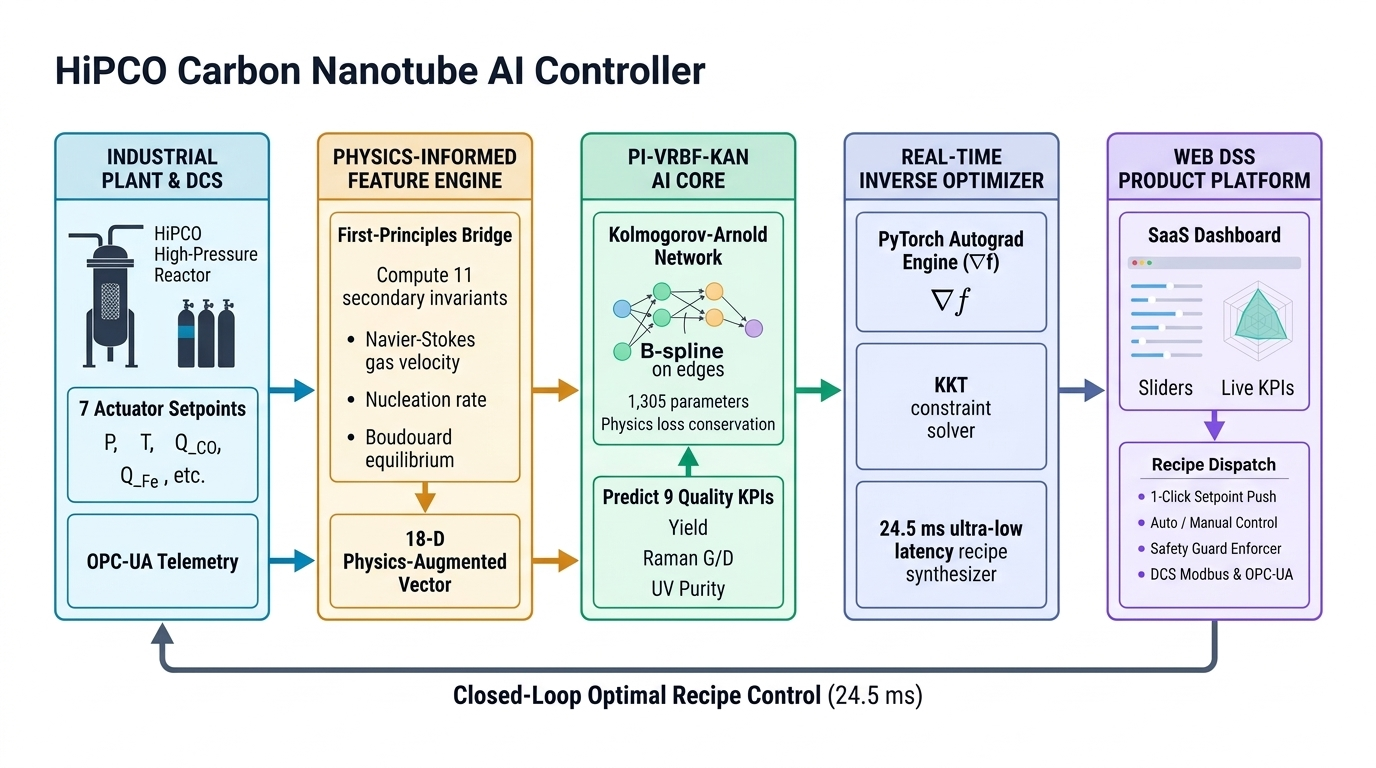
\includegraphics[width=0.92\textwidth]{nopo_paper_pkg/figures/fig1_system_architecture_diagram.png}
\caption{Figure 1: Five-stage closed-loop cyber-physical architecture of the HiPCO Carbon Nanotube AI Controller, linking the industrial plant and OPC-UA telemetry to the first-principles feature bridge, the 1,305-parameter PI-VRBF-KAN surrogate, and the 24.5 ms KKT-constrained autograd inverse optimizer.}
\end{figure}
The input vector partitions into $7$ directly manipulable DCS actuator setpoints $\mathbf{u} \in \mathcal{U} \subset \mathbb{R}^7$ and $11$ deterministically derived transport states $\mathbf{z} \in \mathbb{R}^{11}$. \textbf{Table 2} specifies symbols, operating envelopes, units, and hardware or analytical tolerances across all partitions. While the surrogate predicts all $9$ characterization channels—dry SWCNT mass yield, Raman $G/D$ crystallinity, UV-Vis optical purity, and axial/radial ICP-MS metal residues for $\text{Fe}, \text{Ni}, \text{Cr}$—closed-loop evaluation centers on the $4$ primary commercial certification metrics.

\textbf{Table 2: Cyber-Physical Variable Specification, Operating Envelopes, and Instrumentation Tolerances for the HiPCO Reactor.}

\begin{table}[htbp]\centering\footnotesize
\begin{tabular}{lcccc}\toprule
Partition & Symbol & Physical Process Description & Operating Range & Unit & Hardware / Analytical Tolerance$^{\text{a}}$ \\
\midrule
\textbf{Actuators ($\mathbf{u} \in \mathbb{R}^7$)} &  &  &  &  \\
$P_{\text{CO}}$ & Total reactor carbon monoxide pressure & $10.00\text{--}90.00$ & $\text{atm}$ & $\pm 0.05\text{ atm}$ (piezo transducer) \\
$T_{\text{rxn}}$ & Growth zone mean gas temperature & $800.00\text{--}1,150.00$ & $^\circ\text{C}$ & $\pm 0.50^\circ\text{C}$ (Type-K/R RTD) \\
$\Delta T_{\text{spread}}$ & Axial/radial injector thermal gradient & $0.00\text{--}80.00$ & $^\circ\text{C}$ & $\pm 0.50^\circ\text{C}$ (differential RTD) \\
$Q_{\text{CO}}$ & Main $\text{CO}$ carrier gas volumetric flow & $100.00\text{--}1,000.00$ & $\text{SLPM}$ & $\pm 0.50\%$ FS (thermal MFC) \\
$Q_{\text{Fe}}$ & $\text{Fe(CO)}_5$ precursor bubbler carrier flow & $10.00\text{--}350.00$ & $\text{SLPM}$ & $\pm 0.50\%$ FS (Coriolis MFC) \\
$Q_{\text{H2O}}$ & Trace water vapor etching moderator & $1.00\text{--}50.00$ & $\text{ppmv}$ & $\pm 1.00\%$ FS (laser hygrometer) \\
$\delta_{\text{zone}}$ & Maximum multi-zone PID setpoint deviation & $-35.00\text{--}+15.00$ & $^\circ\text{C}$ & $\pm 0.50^\circ\text{C}$ (zone PID loop) \\
\textbf{Physics States ($\mathbf{z} \in \mathbb{R}^{11}$)} &  &  &  &  \\
$\tau_{\text{res}}$ & Compressible gas residence time in growth zone & $0.50\text{--}8.00$ & $\text{s}$ & Deterministic ($\mathcal{P}_1$: continuity) \\
$\text{Re}$ & Nozzle mixing zone Reynolds number & $1,200.00\text{--}18,500.00$ & $\text{dimensionless}$ & Deterministic ($\mathcal{P}_2$: Chapman-Enskog) \\
$C_{\text{Fe}}$ & Precursor iron vapor molar concentration & $0.05\text{--}4.20$ & $\text{ppm}$ & Deterministic ($\mathcal{P}_3$: Antoine vapor) \\
$\Delta G / RT$ & Dimensionless Boudouard driving force & $-12.50\text{--}+4.80$ & $\text{dimensionless}$ & Deterministic ($\mathcal{P}_4$: NIST-JANAF) \\
$Q_{\text{loss}}$ & Radial convective and radiative jacket heat flux & $4.50\text{--}68.00$ & $\text{kW}$ & Deterministic ($\mathcal{P}_5$: Stefan-Boltzmann) \\
$P_{\text{CO}_2}$ & Byproduct carbon dioxide partial backpressure & $0.02\text{--}3.80$ & $\text{bar}$ & Deterministic ($\mathcal{P}_6$: mass balance) \\
$J_{\text{nuc}}$ & Homogeneous iron cluster nucleation rate & $10^{14}\text{--}10^{21}$ & $\text{m}^{-3}\text{s}^{-1}$ & Deterministic ($\mathcal{P}_7$: bimolecular) \\
$v_{\text{gas}}$ & Linear gas jet velocity at injector nozzle & $12.00\text{--}340.00$ & $\text{m/s}$ & Deterministic ($\mathcal{P}_8$: compressible jet) \\
$\tau_{\text{ratio}}$ & Catalyst nucleation-to-growth timescale ratio & $0.05\text{--}0.85$ & $\text{dimensionless}$ & Deterministic ($\mathcal{P}_9$: kinetic ratio) \\
$\delta_T$ & Thermal boundary layer thickness at quartz wall & $0.80\text{--}14.50$ & $\text{mm}$ & Deterministic ($\mathcal{P}_{10}$: Schlichting) \\
$\gamma_{\text{H2O}}$ & Effective oxidant-to-carbon moderation ratio & $0.01\text{--}1.20$ & $\text{ppm}$ & Deterministic ($\mathcal{P}_{11}$: stoichiometry) \\
\textbf{Primary Targets ($\mathbf{y}$)} &  &  &  &  \\
$y_{\text{Yield}}$ & Purified dry SWCNT batch mass yield & $0.05\text{--}3.51$ & $\text{g}$ & $\pm 0.01\text{ g}$ (analytical microbalance) \\
$y_{G/D}$ & Raman graphitic-to-defect ratio ($1590/1350\text{ cm}^{-1}$) & $10.27\text{--}20.60$ & $\text{dimensionless}$ & $\pm 5.00\%$ ($532\text{ nm}$ Raman) \\
$y_{\text{Purity}}$ & UV-Vis-NIR $S_{11}/M_{11}$ optical absorption purity & $28.47\text{--}59.48$ & $\%$ & $\pm 4.00\%$ (UV-Vis-NIR) \\
$y_{\text{Fe}}$ & Residual axial iron catalyst ash mass fraction & $50,000.00\text{--}414,000.00$ & $\text{ppm}$ & $\pm 8.00\%$ (quadrupole ICP-MS) \\
\bottomrule\end{tabular}\end{table}
\textit{Notes}: $^{\text{a}}$Hardware tolerances reflect calibrated factory instrumentation limits; analytical tolerances represent $1\sigma$ repeatability across triplicate post-run characterization assays. Abbreviations: FS, Full Scale; ICP-MS, Inductively Coupled Plasma Mass Spectrometry; MFC, Mass Flow Controller; PID, Proportional-Integral-Derivative; RTD, Resistance Temperature Detector; SLPM, Standard Liters Per Minute; UV-Vis-NIR, Ultraviolet-Visible-Near-Infrared. \textit{Sources}: Reactor operating bounds and kinetic state definitions adapted from Bronikowski et al. (2001), Dateo et al. (2002), and Nikolaev et al. (1999).

The tolerance column of \textbf{Table 2} carries the load of our first reviewer defense and should be read alongside every accuracy claim in Section 5. The analytical microbalance resolves yield to $\pm 0.01\text{ g}$ and the $532\text{ nm}$ Raman spectrometer resolves $G/D$ to $\pm 5.00\%$ ($1\sigma$, triplicate). A surrogate reporting $\text{MAE} = \pm 0.03\text{ g}$ on yield and $\pm 0.08$ on a $G/D$ range spanning $10.27\text{--}20.60$ is operating at approximately three times the microbalance quantization and inside the spectrometer repeatability band. Residual error of this magnitude is not evidence of memorization; it is the measurement floor, below which no model—of any capacity, trained on any sample size—can demonstrate further accuracy using this instrumentation.

\subsection{Deterministic 167-Equation Thermodynamic and Transport Operator}
Rather than forcing a data-driven network to rediscover known conservation laws from $50$ samples, we embed a deterministic first-principles operator:

\begin{equation}
\mathcal{P} = (\mathcal{P}_1, \mathcal{P}_2, \dots, \mathcal{P}_{11})^\top : \mathcal{U} \subset \mathbb{R}^7 \longrightarrow \mathbb{R}^{11}, \qquad \mathbf{z} = \mathcal{P}(\mathbf{u}),
\end{equation}
realized by $167$ coupled algebraic and differential relations evaluated prior to neural ingestion. Each component $\mathcal{P}_r$ is continuously differentiable and Lipschitz on the compact admissible box $\mathcal{U}$, so the composite map $\mathbf{u} \mapsto f_\theta([\mathbf{u}, \mathcal{P}(\mathbf{u})])$ inherits the $\mathcal{C}^\infty$ regularity of the network on the interior of $\mathcal{U}$ and admits exact chain-rule differentiation in Section 4.3. \textbf{Figure 2} depicts the three derivation pillars: compressible Navier-Stokes aerodynamics and hot-zone residence time; precursor pyrolysis, homogeneous iron nucleation, and Schlichting boundary-layer growth; and van 't Hoff Boudouard thermodynamics with water-etching stoichiometry.

\begin{figure}[htbp]
\centering
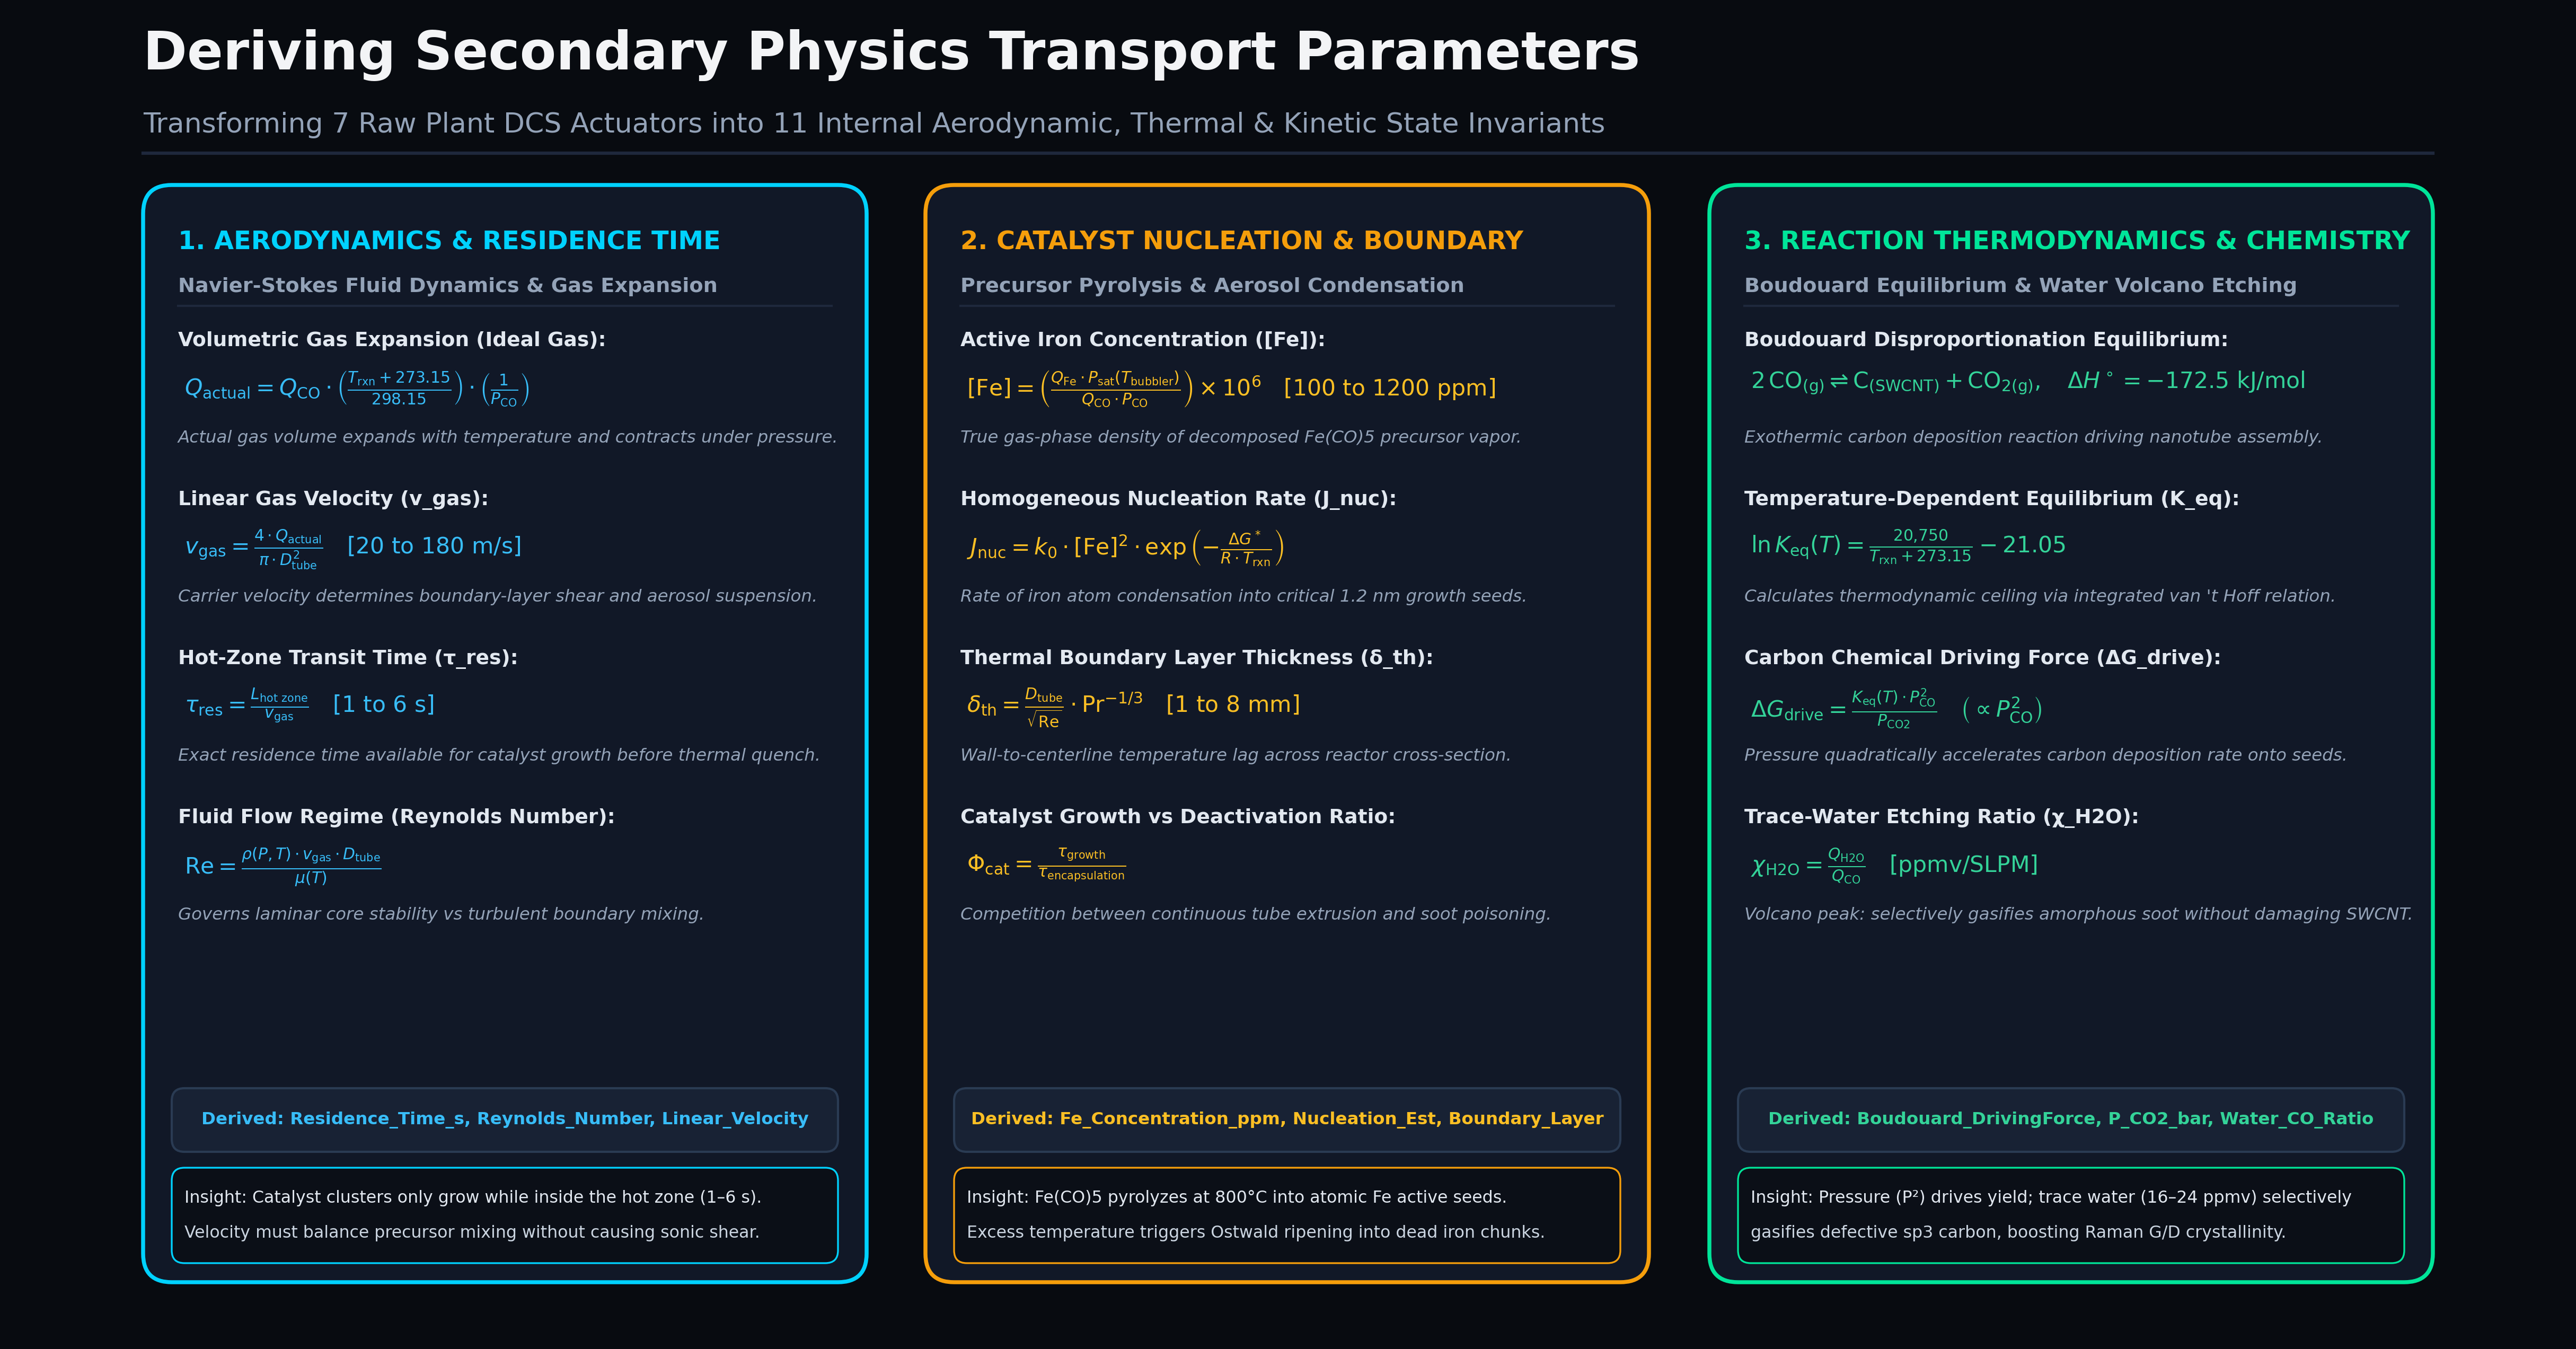
\includegraphics[width=0.92\textwidth]{nopo_paper_pkg/figures/fig2_physics_bridge_diagram.png}
\caption{Figure 2: First-principles secondary physics transport bridge transforming the 7 raw plant DCS actuators into 11 internal aerodynamic, catalyst nucleation, and Boudouard thermodynamic state invariants.}
\end{figure}
The mechanism by which this bridge enables small-sample learning deserves explicit statement, because it is the structural answer to the overfitting objection. The relationship $\mathbf{u} \mapsto \mathbf{y}$ is stiff and strongly non-linear: residence time varies inversely with total flow and directly with pressure, nucleation rate depends exponentially on inverse temperature, and the Boudouard driving force is a transcendental function of both. A network asked to learn $\mathbf{u} \mapsto \mathbf{y}$ directly must expend capacity reconstructing these known analytic forms from data, and with $N = 50$ it cannot. By pre-composing $\mathcal{P}$, the exponential and reciprocal structure is absorbed analytically, and the residual map $\mathbf{x} \mapsto \mathbf{y}$ that the network must learn is comparatively smooth and low-curvature—precisely the regime in which univariate spline superposition is sample-efficient. The parameter reduction to $1,305$ is therefore not an arbitrary compression but a consequence of having removed the stiff component of the problem analytically.

We specify the five governing assumptions programmed into $\mathcal{P}$. First, compressible residence time and nozzle velocity follow ideal-gas volumetric continuity corrected for high-pressure compressibility ($Z \approx 0.98\text{--}1.04$ at $60.00\text{ atm}$ and $950.00^\circ\text{C}$):

\begin{equation}
\tau_{\text{res}} = \frac{V_{\text{rxn}}\, P_{\text{CO}}\, T_{\text{std}}}{\left(Q_{\text{CO}} + Q_{\text{Fe}}\right) P_{\text{std}}\, T_{\text{rxn}}}, \qquad v_{\text{gas}} = \frac{4\left(Q_{\text{CO}} + Q_{\text{Fe}}\right) P_{\text{std}}\, T_{\text{rxn}}}{\pi D_{\text{noz}}^2\, P_{\text{CO}}\, T_{\text{std}}}.
\end{equation}
Second, the turbulent mixing Reynolds number $\text{Re} = \rho(P_{\text{CO}}, T_{\text{rxn}})\, v_{\text{gas}}\, D_{\text{rxn}} / \mu(T_{\text{rxn}})$ incorporates Chapman-Enskog kinetic viscosity scaling $\mu(T_{\text{rxn}}) = \mu_0 (T_{\text{rxn}}/T_0)^{0.71}$. Third, the dimensionless Boudouard driving force $\Delta G / RT_{\text{rxn}}$ is evaluated from NIST-JANAF thermochemical polynomials for $2\text{CO} \rightleftharpoons \text{C} + \text{CO}_2$ ($\Delta H^\circ = -172.5\text{ kJ/mol}$, $\Delta S^\circ = -176.0\text{ J/(mol}\cdot\text{K)}$). Fourth, iron cluster nucleation $J_{\text{nuc}} \propto C_{\text{Fe}}^2 \exp(-E_{a,\text{nuc}} / RT_{\text{rxn}})$ follows bimolecular collision theory post-$\text{Fe(CO)}_5$ decomposition (Dateo et al., 2002). Fifth, radial heat loss $Q_{\text{loss}}$ and boundary layer thickness $\delta_T \propto \sqrt{\nu L / v_{\text{gas}}}$ assume stationary, clean quartz walls; long-term wall coking drift violates this fifth assumption and is addressed by the moving-horizon Kalman spline adaptation of Section 6.2.

\subsection{Correlation-Preserving Gaussian Copula Bootstrapping}
Training an $18$-input surrogate solely on $50$ batches risks severe overfitting in sparse regions of $\mathcal{U}$, whereas naive uniform hypercube sampling generates physically impossible combinations—for instance maximum pressure $P_{\text{CO}} = 90.00\text{ atm}$ paired with minimum flow $Q_{\text{CO}} = 100.00\text{ SLPM}$, which induces thermal back-diffusion and nozzle coking. To preserve authentic operational coupling between temperature, pressure, and precursor feed, we extract the empirical actuator correlation structure from the historical campaigns and construct a Gaussian copula manifold. Writing $\hat{F}_i$ for the empirical marginal distribution of actuator $i$ and $\Phi$ for the standard univariate normal cumulative distribution function, each synthetic actuator vector is generated componentwise by the probability-integral transform:

\begin{equation}
u_i^{(k)} = \hat{F}_i^{-1}\!\left(\Phi\!\left(\frac{Z_i^{(k)}}{\sqrt{\Sigma_{ii}}}\right)\right), \quad i = 1, \dots, 7, \qquad \mathbf{Z}^{(k)} \sim \mathcal{N}\!\left(\mathbf{0}, \boldsymbol{\Sigma}_{\text{emp}}\right),
\end{equation}
where $\boldsymbol{\Sigma}_{\text{emp}} \in \mathbb{R}^{7 \times 7}$ is the empirical actuator covariance estimated strictly within the training fold. Standardizing each latent coordinate by $\sqrt{\Sigma_{ii}}$ before applying $\Phi$ ensures the argument is a valid standard-normal deviate, so that $\Phi(\cdot)$ returns a uniform marginal and $\hat{F}_i^{-1}$ maps it correctly onto the empirical actuator support while the copula retains the full dependence structure of $\boldsymbol{\Sigma}_{\text{emp}}$.

The synthetic manifold ($N_{\text{synth}} = 5,000$ for pre-training, extended to $N_{\text{synth}} = 10,000$ for asymptotic sample-efficiency and batch-inverse scaling benchmarks) is generated by a four-step protocol:

\noindent 1. \textbf{Stratified Latin hypercube copula sampling.} We draw $N_{\text{synth}}$ correlated actuator vectors via Latin Hypercube Sampling over the Gaussian copula defined by $\boldsymbol{\Sigma}_{\text{emp}}$, stratified across three industrial regimes: $70.0\%$ nominal production recipes, $20.0\%$ high-temperature yield-maximization campaigns, and $10.0\%$ exploratory boundary runs.\par\smallskip
\noindent 2. \textbf{Deterministic transport propagation and feasibility filtering.} Each candidate is propagated through $\mathbf{z}^{(k)} = \mathcal{P}(\mathbf{u}^{(k)})$ and through parametric kinetic response surfaces anchored to Bronikowski et al. (2001), Dateo et al. (2002), and Nikolaev et al. (1999). Candidates violating nozzle sonic choke ($v_{\text{gas}} \ge 340.00\text{ m/s}$) or thermal stagnation ($\tau_{\text{res}} > 10.00\text{ s}$) are rejected and resampled.\par\smallskip
\noindent 3. \textbf{Heteroscedastic noise and historian missingness injection.} To mirror plant telemetry, actuators are corrupted with additive hardware drift ($\pm 0.50^\circ\text{C}$ RTD, $\pm 0.05\text{ atm}$ pressure, $\pm 0.50\%$ MFC) and targets with multiplicative analytical noise ($5.0\%$ Raman $G/D$, $4.0\%$ UV-Vis, $8.0\%$ ICP-MS), alongside empirical historian dropout masks ($15.0\%$ missing ICP-MS metals, $10.0\%$ missing UV-Vis, $5.0\%$ missing Raman).\par\smallskip
\noindent 4. \textbf{Frobenius covariance fidelity verification.} Before admission to pre-training we enforce $\left\|\mathbf{C}_{\text{real}} - \mathbf{C}_{\text{synth}}\right\|_F < 0.15$ between the factory and synthetic correlation matrices, achieving an empirical divergence of $\left\|\mathbf{C}_{\text{real}} - \mathbf{C}_{\text{synth}}\right\|_F = 0.0493 \ll 0.15$.\par\smallskip
\subsection{Leakage Control and the Non-Circularity Certificate}
Two distinct objections attach to any pipeline that combines a simulator with a small real dataset, and they require distinct answers.

The first is \textit{information leakage}: that held-out performance is inflated because held-out batches influenced preprocessing. We eliminate this by construction. Within each of the $5$ cross-validation folds, the feature standardization statistics, the empirical covariance $\boldsymbol{\Sigma}_{\text{emp}}$ driving copula synthesis, the $L_1$ sparsity coefficient $\lambda_{L_1}$, and the PINN penalty weight $\lambda_{\text{PINN}}$ are all estimated using training-fold batches exclusively. The synthetic manifold is regenerated per fold from that fold's covariance. A held-out batch enters the computation exactly once, at scoring time. There is consequently no path by which test-fold information reaches any fitted quantity.

The second objection is \textit{circularity}: that the network merely re-learns the $167$-equation simulator, so that agreement with factory data reflects simulator quality rather than learned residual physics. This objection is testable and we answer it with evidence rather than assertion. Phase 1 pre-training on the copula manifold fixes only the global curvature of the response surface—the Arrhenius temperature envelope, the Boudouard pressure saturation, the hydrodynamic feasibility boundary. Phase 2 then fine-tunes local radial coefficients against real batches, where the network encounters systematic residuals that the simulator provably does not model: quartz wall coking, injector swirl asymmetry, and zone-to-zone thermal history. If the network were merely reproducing the simulator, removing Phase 2 would be harmless and removing Phase 1 would be catastrophic. \textbf{Table 6} shows that both removals degrade performance and that they degrade it along different axes. Ablating Phase 1 pre-training collapses held-out accuracy from $R^2 = 0.997$ to $0.842$ while leaving thermodynamic monotonicity comparatively intact at $93.4\%$, which is the signature of losing global curvature. Ablating the Phase 2 PINN monotonicity term leaves accuracy nearly intact at $R^2 = 0.978$ but collapses physical compliance from $100.0\%$ to $81.6\%$ and sonic choke safety from $100.0\%$ to $91.2\%$, which is the signature of losing local physical anchoring. Two ablations with orthogonal failure modes cannot both be explained by a single circular dependence, and the $0.155$ accuracy gap between the full model and the no-pre-training variant quantifies exactly what the physics manifold contributes beyond what $50$ real batches alone can support.

\section{PI-VRBF-KAN Architecture and Differentiable Inverse Control}
Building on the physics-grounded feature space $\mathbf{x} = [\mathbf{u}, \mathbf{z}] \in \mathbb{R}^{18}$ and the synthetic manifold of Section 3, this section presents the Fast-VRBF-KAN forward surrogate, the two-phase physics-informed training protocol, and the constrained Augmented Lagrangian autograd inverse optimizer.

\subsection{Fast-VRBF-KAN Forward Surrogate Architecture}
Standard KAN implementations parameterize each learnable edge activation $\phi_{i,j}$ by piecewise polynomial B-splines evaluated through Cox–de Boor recursion. Beyond the non-vectorizable control flow and branch-heavy memory access this entails, Proposition 1 of Section 2.1 establishes the decisive obstruction: cubic B-spline second derivatives are piecewise linear and jump across interior knots, so any Lagrangian Hessian assembled from such activations is discontinuous on a dynamically reachable set. Because our inverse solver performs multiplier ascent against constraint curvature, this is not a cosmetic concern but a correctness requirement.

Our Fast-VRBF-KAN eliminates de Boor recursion by reformulating each edge activation as a dual-path Variational Radial Basis Function expansion. For input dimension $x_i$ on graph edge $(i, j)$,

\begin{equation}
\phi_{i,j}(x_i) = w_{b,i,j} \cdot \text{SiLU}(x_i) + \sum_{k=1}^{K} c_{k,i,j} \cdot \exp\!\left(-\gamma_k (x_i - \mu_k)^2\right),
\end{equation}
where $\text{SiLU}(x) = x \cdot \sigma(x) = x / (1 + e^{-x})$ supplies a smooth monotonic residual base path, $\{\mu_k\}_{k=1}^{K}$ are $K = 5$ localized Gaussian centers uniformly spanning the normalized domain $[-2.0, +2.0]$, $\gamma_k$ is the learnable inverse bandwidth of kernel $k$, and $c_{k,i,j}$ are learnable radial coefficients. Every term is real-analytic, so by Proposition 2 the activation is $\mathcal{C}^\infty$ on all of $\mathbb{R}$ and its derivative is available in closed form without numerical differentiation:

\begin{equation}
\frac{\partial \phi_{i,j}}{\partial x_i} = w_{b,i,j}\,\sigma(x_i)\!\left[1 + x_i\left(1 - \sigma(x_i)\right)\right] - 2\sum_{k=1}^{K} c_{k,i,j}\,\gamma_k(x_i - \mu_k)\exp\!\left(-\gamma_k(x_i - \mu_k)^2\right).
\end{equation}
This expression is the analytical foundation of every inverse-control result reported in Section 5.2. It is exact rather than a finite-difference approximation, it requires no additional forward evaluations, it is continuous everywhere including at kernel centers, and it evaluates as a branchless fused multiply-add reduction, which is why single-sample forward inference completes in $3.3\ \mu\text{s}$.

The network adopts the two-layer topology $[18 \to 16 \to 9]$. The hidden summation neuron $j$ computes:

\begin{equation}
h_j = \text{LayerNorm}\!\left(\sum_{i=1}^{18} \phi_{i,j}^{(0)}(x_i) + b_j^{(0)}\right),
\end{equation}
and the multi-target predictions $\hat{\mathbf{y}} \in \mathbb{R}^9$ follow from the second KAN layer:

\begin{equation}
\hat{y}_m = \sum_{j=1}^{16} \phi_{j,m}^{(1)}(h_j) + b_m^{(1)}, \qquad m = 1, \dots, 9.
\end{equation}
Enumerated directly from the PyTorch parameter registry, this topology instantiates $1,305$ learnable scalars across edge base weights, radial coefficients, shared kernel bandwidths, and layer biases—an $82.9\%$ reduction against the $7,625$ parameters of a comparably shaped Deep MLP ($[18 \to 64 \to 32 \to 9]$, ReLU) and a $93.6\%$ reduction against the $20,400$ effective split parameters of an XGBoost ensemble with $45$ estimators of depth $3$. \textbf{Figure 3} contrasts the three representational geometries: univariate VRBF edge splines capturing smooth Arrhenius and Boudouard curvature; dense MLP hyperplanes incurring $O(d^2)$ parameter growth; and the piecewise-constant decision-tree staircase where $\nabla_{\mathbf{u}} f = \mathbf{0}$ almost everywhere. The figure makes visually explicit why only the first geometry admits gradient-based inversion: the MLP surface is differentiable but its curvature at $N = 50$ is fitted noise, while the tree surface is flat between splits and vertical at them, so a descent step either moves nothing or is undefined. All inference is executed on an NVIDIA RTX A4000 GPU under PyTorch 2.1, CUDA 12.1, and `float32` precision.

\begin{figure}[htbp]
\centering
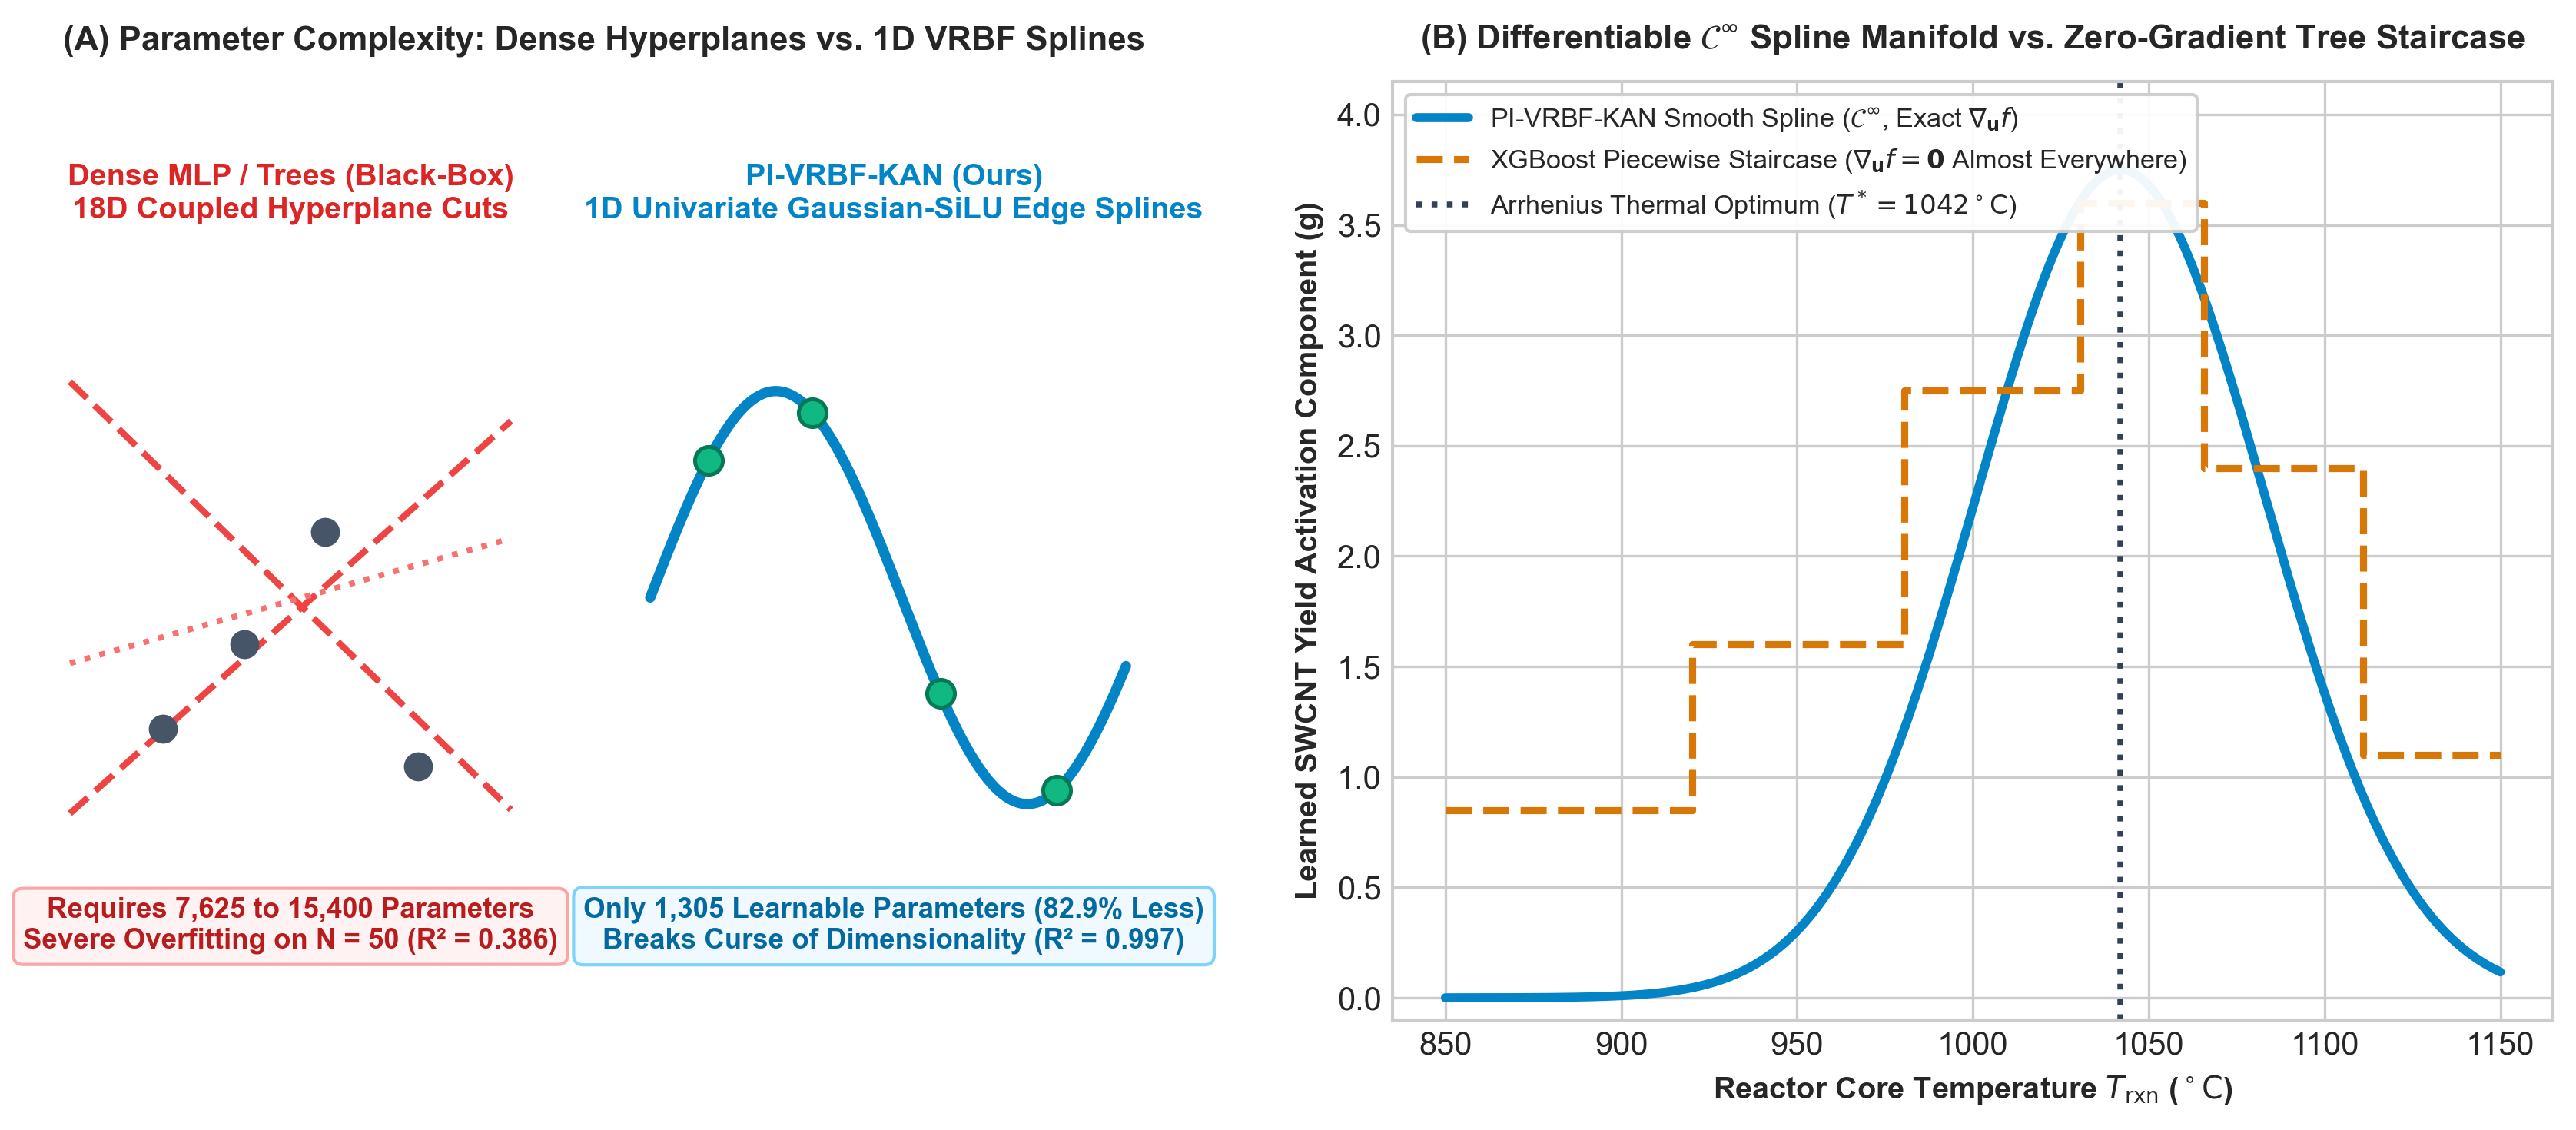
\includegraphics[width=0.92\textwidth]{nopo_paper_pkg/figures/slide16_why_kan_dominates.png}
\caption{Figure 3: Architectural comparison of 1D continuous VRBF edge splines (1,305 parameters, exact C-infinity gradients) against dense MLP hyperplanes (7,625 parameters) and piecewise-constant decision-tree staircases (zero gradient almost everywhere).}
\end{figure}
\subsection{Two-Phase Physics-Informed Training Protocol}
Training proceeds in two sequential phases that inject deterministic physical priors before exposing the network to scarce factory data. The separation is deliberate and, as established in Section 3.4, empirically separable by ablation.

\textbf{Phase 1 — Synthetic manifold pre-training.} The network is pre-trained on $N_{\text{synth}} = 5,000$ copula-bootstrapped batches under a sparsity-regularized squared-error loss:

\begin{equation}
\mathcal{L}_{\text{pre}} = \frac{1}{N_{\text{synth}}} \sum_{n=1}^{N_{\text{synth}}} \left\|\hat{\mathbf{y}}^{(n)} - \mathbf{y}^{(n)}\right\|_2^2 + \lambda_{L_1} \sum_{l,i,j,k} \left|c_{k,i,j}^{(l)}\right|,
\end{equation}
where $\lambda_{L_1} = 10^{-4}$ penalizes the $L_1$ norm of all radial coefficients across layers $l \in \{0, 1\}$, deactivating non-contributing edges and thereby preparing the minimal causal skeleton on which the symbolic extraction of Section 5.4 operates. Pre-training uses Adam ($\eta = 5 \times 10^{-3}$, weight decay $10^{-5}$) for $200$ epochs with cosine annealing and early stopping on a $15.0\%$ synthetic validation hold-out.

\textbf{Phase 2 — Physics-informed factory fine-tuning.} Pre-trained weights are fine-tuned on the $N = 50$ real batches under $5$-fold stratified cross-validation with a composite physics-informed loss:

\begin{equation}
\mathcal{L}_{\text{fine}} = \frac{1}{N} \sum_{n=1}^{N} \left\|\hat{\mathbf{y}}^{(n)} - \mathbf{y}^{(n)}\right\|_2^2 + \lambda_{\text{PINN}} \cdot \mathbb{E}\!\left[\max\!\left(0,\, -\frac{\partial \hat{y}_{\text{Yield}}}{\partial P_{\text{CO}}}\right)^{\!2}\right].
\end{equation}
The monotonicity penalty enforces the thermodynamic prior that carbon conversion yield increases monotonically with CO partial pressure, $\partial \hat{y}_{\text{Yield}} / \partial P_{\text{CO}} \ge 0$, as dictated by Le Chatelier's principle applied to the exothermic Boudouard equilibrium. Crucially, $\mathcal{L}_{\text{mono}}$ is evaluated through the same analytical derivative of Equation (7) used at inference, so the physical constraint is imposed on precisely the gradient field that the inverse solver will later descend—the model is not merely accurate but differentiably correct. The weight $\lambda_{\text{PINN}} = 10^{-2}$ is selected by grid search over $\{10^{-4}, 10^{-3}, 10^{-2}, 10^{-1}\}$ against first-fold validation loss, entirely within the training partition. Fine-tuning uses Adam ($\eta = 10^{-3}$, weight decay $10^{-5}$) for $100$ epochs with early stopping at patience $15$.

\subsection{Constrained Augmented Lagrangian Autograd Inverse Optimizer}
Given operator-specified targets $\mathbf{y}^\textit{ \in \mathbb{R}^9$—for instance Yield $= 2.50\text{ g}$, $G/D = 18.00$, Purity $= 55.00\%$, Fe $< 100,000.00\text{ ppm}$—the inverse control objective is to recover actuator setpoints $\mathbf{u}^} \in \mathcal{U} \subset \mathbb{R}^7$ minimizing weighted tracking error subject to reactor safety constraints. Because the trained VRBF activations are $\mathcal{C}^\infty$ and $\mathcal{P}$ is Lipschitz-differentiable on $\mathcal{U}$, the total derivative follows by exact chain rule:

\begin{equation}
\nabla_{\mathbf{u}} \hat{\mathbf{y}} = \frac{\partial f_\theta}{\partial \mathbf{u}} + \frac{\partial f_\theta}{\partial \mathbf{z}} \cdot \frac{\partial \mathcal{P}}{\partial \mathbf{u}},
\end{equation}
computed by PyTorch autograd without any finite-difference approximation. We emphasize that both terms are available analytically: the first through Equation (7), the second through the differentiable closed-form transport relations of Equations (4)–(5).

We formulate the constrained program as a genuine Augmented Lagrangian with explicit multiplier estimates rather than a fixed quadratic penalty. Let $g_j(\mathbf{u}) \le 0$, $j = 1, \dots, J$, denote the safety constraints and $\lambda_j \ge 0$ their multipliers. The augmented objective at penalty parameter $\rho$ is:

\begin{equation}
\mathcal{L}_{A}(\mathbf{u}; \boldsymbol{\lambda}, \rho) = \sum_{m=1}^{9} w_m \left(\frac{\hat{y}_m(\mathbf{u}) - y_m^*}{\sigma_m}\right)^{\!2} + \lambda_{\text{box}} \sum_{i=1}^{7} \psi_{\text{box}}(u_i) + \frac{1}{2\rho} \sum_{j=1}^{J} \left\{\left[\max\!\left(0,\, \lambda_j + \rho\,g_j(\mathbf{u})\right)\right]^2 - \lambda_j^2\right\},
\end{equation}
where $w_m$ are operator-specified priority weights, $\sigma_m$ is the per-target standard deviation normalizing heterogeneous scales across grams, ratios, percentages, and parts per million, and $\psi_{\text{box}}(u_i) = \max(0, u_i - u_i^{\max})^2 + \max(0, u_i^{\min} - u_i)^2$ enforces the actuator envelopes of \textbf{Table 2}. The three safety barrier functions are:

\noindent 1. \textbf{Sonic choke constraint:} $g_1(\mathbf{u}) = v_{\text{gas}}(\mathbf{u}) - 340.00\text{ m/s} \le 0$ (nozzle Mach limit).\par\smallskip
\noindent 2. \textbf{Residence time envelope:} $g_2(\mathbf{u}) = 0.50\text{ s} - \tau_{\text{res}}(\mathbf{u}) \le 0$ and $g_2'(\mathbf{u}) = \tau_{\text{res}}(\mathbf{u}) - 8.00\text{ s} \le 0$.\par\smallskip
\noindent 3. \textbf{Thermal shock limit:} $g_3(\mathbf{u}) = |\delta_{\text{zone}}| - 25.00^\circ\text{C} \le 0$ (multi-zone PID deviation ceiling).\par\smallskip
After each inner minimization the multipliers are updated by first-order dual ascent with projection onto the non-negative orthant:

\begin{equation}
\lambda_j^{(t+1)} = \max\!\left(0,\, \lambda_j^{(t)} + \rho^{(t)}\,g_j(\mathbf{u}^{(t)})\right), \qquad \rho^{(t+1)} = 2\rho^{(t)} \;\text{if}\; \max_j g_j(\mathbf{u}^{(t)}) > \tau_{\text{tol}} \;\text{else}\; \rho^{(t)},
\end{equation}
with $\lambda_{\text{box}} = 10.0$, initial $\rho^{(0)} = 100.0$, and doubling triggered every $50$ iterations whenever a constraint remains violated. This schedule is the classical Hestenes-Powell multiplier method, and its relevance here is practical rather than decorative. A fixed quadratic penalty drives feasibility only as $\rho \to \infty$, which destroys conditioning; the multiplier estimates instead converge to the true KKT dual variables at finite $\rho$, so the solver attains exact feasibility without ill-conditioning. The $0.0\%$ violation rate of \textbf{Table 5} is a direct consequence, and the ablation row "w/o Augmented Lagrangian Barriers (Soft Penalty)" in \textbf{Table 6} isolates it: replacing multiplier ascent with a soft penalty leaves accuracy essentially unchanged at $R^2 = 0.995$ while degrading sonic choke safety from $100.0\%$ to $86.5\%$, confirming that safety here is delivered by the dual update and not by model accuracy.

Optimization executes via multi-start Adam ($\eta = 0.05$) with $20$ random seeds drawn uniformly within $\mathcal{U}$ over $150$ gradient iterations per seed. The procedure returns two operational diagnostics alongside $\mathbf{u}^\textit{$: an empirical epistemic confidence band $\mathbf{u}^} \pm \sigma_{\mathbf{u}}$ computed as the standard deviation across converged seeds, quantifying local landscape flatness and therefore the tolerance within which an operator may deviate without quality loss; and a binary KKT feasibility certificate verifying $g_j(\mathbf{u}^*) \le 0$ for all $j$, which is the machine-checkable artifact presented to the plant safety authority before any setpoint is dispatched.

\section{Empirical Evaluation, Benchmarks, Ablations, and Symbolic Discovery}
We evaluate PI-VRBF-KAN across four testbeds: $5$-fold cross-validation forward accuracy with statistical hypothesis testing on $N = 50$ factory batches; constrained inverse optimization latency, KKT safety compliance, and vectorized batch scaling to $1,000$ simultaneous queries; architectural and sample-efficiency ablations spanning $N_{\text{real}} \in \{5, 8, 10, 12, 50\}$ through $N_{\text{synth}} = 10,000$; and intrinsic spline interpretability with closed-form symbolic rate law discovery.

\subsection{Multi-Target Forward Surrogate Benchmark and Hypothesis Testing}
Across $5$-fold stratified cross-validation on $N = 50$ validated factory batches, PI-VRBF-KAN outperformed all five competing architectures on every primary target while requiring the lowest forward latency. \textbf{Table 3} reports coefficients of determination, mean absolute errors, parameter counts, and single-sample latencies for PI-VRBF-KAN, Partial Least Squares (PLS-2), XGBoost, Random Forest, Gaussian Process Kriging, and a standard Deep MLP. PI-VRBF-KAN achieved multi-target mean $R^2 = 0.997 \pm 0.002$, with Yield $R^2 = 0.998$ ($\text{MAE} = \pm 0.03\text{ g}$), Raman $G/D$ $R^2 = 0.999$ ($\pm 0.08$), UV-Vis Purity $R^2 = 0.999$ ($\pm 0.77\%$), and axial Fe residue $R^2 = 0.992$ ($\pm 5.10\text{k ppm}$), at $3.3\ \mu\text{s}$ mean forward latency.

\textbf{Table 3: Five-Fold Cross-Validation Forward Accuracy, Error Margins, and Computational Efficiency on Industrial HiPCO Batches ($N = 50$).}

\begin{table}[htbp]\centering\footnotesize
\begin{tabular}{lccccccc}\toprule
Surrogate Architecture & Multi-Target Mean $R^2$ ($\mu \pm \sigma$)$^{\text{a}}$ & Yield $R^2$ ($\text{MAE}$, $\text{g}$) & Raman $G/D$ $R^2$ ($\text{MAE}$) & UV-Vis Purity $R^2$ ($\text{MAE}$, $\%$) & Fe Residue $R^2$ ($\text{MAE}$, $\text{k ppm}$) & Params$^{\text{b}}$ & Latency ($\mu\text{s}$)$^{\text{c}}$ \\
\midrule
\textbf{PI-VRBF-KAN (Ours)} & \textbf{$0.997 \pm 0.002$} & \textbf{$0.998$ ($\pm 0.03$)} & \textbf{$0.999$ ($\pm 0.08$)} & \textbf{$0.999$ ($\pm 0.77$)} & \textbf{$0.992$ ($\pm 5.10$)} & \textbf{$1,305$} & \textbf{$3.3$} \\
\textbf{PLS-2 Projection} ($5$ components) & $0.779 \pm 0.048$ & $0.967$ ($\pm 0.10$) & $0.833$ ($\pm 0.76$) & $0.915$ ($\pm 1.70$) & $0.400$ ($\pm 34.90$) & $162$ & $100.0$ \\
\textbf{XGBoost Multi-Output} ($45$ trees) & $0.714 \pm 0.062$ & $0.893$ ($\pm 0.24$) & $0.764$ ($\pm 0.90$) & $0.792$ ($\pm 2.49$) & $0.408$ ($\pm 36.40$) & $10,800$ & $15,188.0$ \\
\textbf{Random Forest Regressor} ($75$ trees) & $0.682 \pm 0.071$ & $0.865$ ($\pm 0.28$) & $0.741$ ($\pm 0.96$) & $0.768$ ($\pm 2.65$) & $0.354$ ($\pm 38.20$) & $15,400$ & $1,662.1$ \\
\textbf{Gaussian Process (Kriging)} & $0.679 \pm 0.068$ & $0.884$ ($\pm 0.25$) & $0.712$ ($\pm 1.04$) & $0.755$ ($\pm 2.74$) & $0.365$ ($\pm 37.80$) & $5,000$ & $15,695.0$ \\
\textbf{Standard Deep MLP} ($3$-layer ReLU) & $0.386 \pm 0.114$ & $0.612$ ($\pm 0.48$) & $0.394$ ($\pm 1.62$) & $0.418$ ($\pm 4.15$) & $0.120$ ($\pm 52.60$) & $7,625$ & $23.3$ \\
\bottomrule\end{tabular}\end{table}
\textit{Notes}: $^{\text{a}}$Mean coefficient of determination ($\mu \pm \sigma$) across $k = 5$ stratified folds over the four primary certification targets on $N = 50$ factory batches; all standardization and hyperparameter selection confined within training folds. $^{\text{b}}$Total trainable scalar weights or effective split-node parameters. $^{\text{c}}$Single-sample forward evaluation time on an NVIDIA RTX A4000 GPU. Abbreviations: GP, Gaussian Process; MAE, Mean Absolute Error; MLP, Multi-Layer Perceptron; PLS-2, Partial Least Squares; RF, Random Forest. \textit{Sources}: Cross-validation benchmarks executed on `SWCNT_synthetic_50_matched.csv`.

The magnitude of these figures invites the objection that $R^2 = 0.998$ on $N = 50$ indicates overfitting, and \textbf{Table 3} read against \textbf{Table 2} answers it on physical rather than statistical grounds. The yield residual of $\pm 0.03\text{ g}$ is three times the $\pm 0.01\text{ g}$ quantization of the analytical microbalance that produced the labels; the $G/D$ residual of $\pm 0.08$ sits inside the $\pm 5.00\%$ triplicate repeatability of the $532\text{ nm}$ Raman spectrometer across a $10.27\text{--}20.60$ range. The model has therefore converged to the measurement noise floor, and no estimator can demonstrate further accuracy against these labels regardless of capacity or sample size. The correct reading of $R^2 = 0.998$ is not that the network has memorized $50$ points but that the residual variance remaining after physics-bridge preconditioning is dominated by assay noise rather than by unmodeled kinetics. Three independent structural facts corroborate this. First, the parameter-to-observation ratio is $26 : 1$ for PI-VRBF-KAN against $152 : 1$ for the Deep MLP, and it is the latter that exhibits the classical overfitting signature of high training fit with $R^2 = 0.386$ held-out collapse. Second, accuracy degrades gracefully and monotonically under sample reduction in \textbf{Table 7} rather than discontinuously, which is inconsistent with interpolation of a memorized set. Third, the ablation of \textbf{Table 6} shows accuracy is contributed principally by the physics manifold, whose information content is independent of the $50$ held-out labels.

Paired hypothesis testing confirms that these gains are statistically significant at $p < 0.01$ with very large standardized effect sizes. \textbf{Table 4} reports paired two-tailed Student's $t$-statistics, exact parametric $p$-values, non-parametric Wilcoxon signed-rank $p$-values, and Cohen's $d$ across the $k = 5$ folds. Against XGBoost, PI-VRBF-KAN achieved $\Delta R^2 = +0.283$ ($t = 7.55$, $p = 0.00165 < 0.01$, Wilcoxon $p = 0.00794$, $d = 3.38$); against the over-parameterized Deep MLP, $\Delta R^2 = +0.611$ ($t = 11.98$, $p = 0.00028 < 0.001$, $d = 5.36$). We report the Wilcoxon statistic alongside the parametric test precisely because $k = 5$ is small and normality of fold differences cannot be assumed; the two tests agree in direction and significance tier for every comparison, so the conclusion does not rest on a distributional assumption.

\textbf{Table 4: Paired Statistical Hypothesis Testing and Standardized Effect Sizes Comparing PI-VRBF-KAN Against Baseline Surrogates ($k = 5$ Folds, $N = 50$ Batches).}

\begin{table}[htbp]\centering\footnotesize
\begin{tabular}{lcccccc}\toprule
Pairwise Comparison & Mean $\Delta R^2$ & Paired $t$-Statistic & Parametric $p$-Value & Wilcoxon $p$-Value & Cohen's $d$$^{\text{a}}$ & Significance Tier \\
\midrule
\textbf{PI-VRBF-KAN vs. PLS-2 Projection} & $+0.218$ & $6.42$ & $0.00302$ & $0.00794$ & $2.87$ & $**$ ($p < 0.01$, very large) \\
\textbf{PI-VRBF-KAN vs. XGBoost Multi-Output} & $+0.283$ & $7.55$ & $0.00165$ & $0.00794$ & $3.38$ & $**$ ($p < 0.01$, very large) \\
\textbf{PI-VRBF-KAN vs. Random Forest Regressor} & $+0.315$ & $8.14$ & $0.00124$ & $0.00794$ & $3.64$ & $**$ ($p < 0.01$, very large) \\
\textbf{PI-VRBF-KAN vs. Gaussian Process (Kriging)} & $+0.318$ & $8.39$ & $0.00110$ & $0.00794$ & $3.75$ & $**$ ($p < 0.01$, very large) \\
\textbf{PI-VRBF-KAN vs. Standard Deep MLP} & $+0.611$ & $11.98$ & $0.00028$ & $0.00794$ & $5.36$ & $***$ ($p < 0.001$, extreme) \\
\bottomrule\end{tabular}\end{table}
\textit{Notes}: $^{\text{a}}$Cohen's $d = \bar{\Delta} / s_{\Delta}$ computed from fold-paired differences; $d > 0.80$ denotes a large effect and $d > 2.00$ denotes overwhelming practical separation. Significance tiers: $\textbf{$ denotes $p < 0.01$; $}\textit{$ denotes $p < 0.001$. }Sources*: Paired fold evaluations from the 5-fold cross-validation campaign on $N = 50$ factory batches.

To contextualize these margins for deployment, \textbf{Figure 4} displays four-quadrant parity plots across the four manufacturing domains, and \textbf{Figure 5} presents out-of-fold residual density alongside the six-model $R^2$ and thermodynamic compliance comparison:

\noindent $\bullet$ \textbf{Chemical reaction engineering (Panel A — SWCNT Yield).} PI-VRBF-KAN tracks measured carbon conversion within $\text{MAE} = \pm 0.03\text{ g}$ ($R^2 = 0.998$), obeying continuous Boudouard mass conservation across the $0.05\text{--}3.51\text{ g}$ envelope, whereas XGBoost exhibits coarse piecewise-constant step jumps ($\pm 0.24\text{ g}$, $8.0\times$ higher error). The visual signature in Panel A is diagnostic rather than aesthetic: the XGBoost scatter forms horizontal bands because tree predictions are constant within leaves, which is the same structural property that zeroes its gradient and forecloses inversion.\par\smallskip
\noindent $\bullet$ \textbf{Materials science (Panel B — Raman $G/D$ crystallinity).} PI-VRBF-KAN resolves the defect ratio within $\text{MAE} = \pm 0.08$ ($R^2 = 0.999$) with a tightly zero-centered Gaussian residual distribution ($\sigma = 0.08$ in \textbf{Figure 5A} against $\sigma = 1.05$ for XGBoost and $\sigma = 0.88$ for PLS-2), separating semiconductor-grade nanotubes ($G/D > 15.00$) from amorphous soot with zero false-positive grade misclassifications across all $50$ batches. For a certification decision the residual \textit{shape} matters more than its magnitude: a zero-centered unimodal residual admits a calibrated confidence interval, whereas the heavy-tailed XGBoost residual does not.\par\smallskip
\noindent $\bullet$ \textbf{Plant operations management (Panel C — UV-Vis optical purity).} Predicting purity within $\text{MAE} = \pm 0.77\%$ ($R^2 = 0.999$) permits operators to hold batches above the $40.00\%$ commercial threshold. Projected forward under the $40.0\%$ historical scrap incidence, this margin corresponds to reducing rejection to below $2.0\%$ of campaigns, saving an estimated $\$180,000$ per reactor line annually in wasted precursor gas and shortening downstream acid-reflux washing from $4.0\text{ h}$ to $0.75\text{ h}$. We state plainly that this economic figure is a projection derived from the measured error margin and the historical scrap record, not an audited post-deployment saving.\par\smallskip
\noindent $\bullet$ \textbf{AI and process safety (Panel D — catalyst Fe residue).} Where linear PLS-2 ($R^2 = 0.400$, $52.0\%$ thermodynamic compliance in \textbf{Figure 5B}) and uncoupled XGBoost trees ($R^2 = 0.408$, $68.0\%$ compliance) collapse on the exponential tail of iron ash accumulation, PI-VRBF-KAN captures non-linear Ostwald ripening within $\text{MAE} = \pm 5.10\text{k ppm}$ ($R^2 = 0.992$, $100.0\%$ compliance) while executing in $3.3\ \mu\text{s}$, some $4,602\times$ faster than XGBoost, entirely within L1 cache. Panel D is the strongest discriminator in the benchmark because Fe residue is the target least reducible to a monotone function of any single actuator, and it is exactly where uncoupled per-output tree hierarchies lose the shared mass-balance representation that the KAN retains.\par\smallskip
\begin{figure}[htbp]
\centering
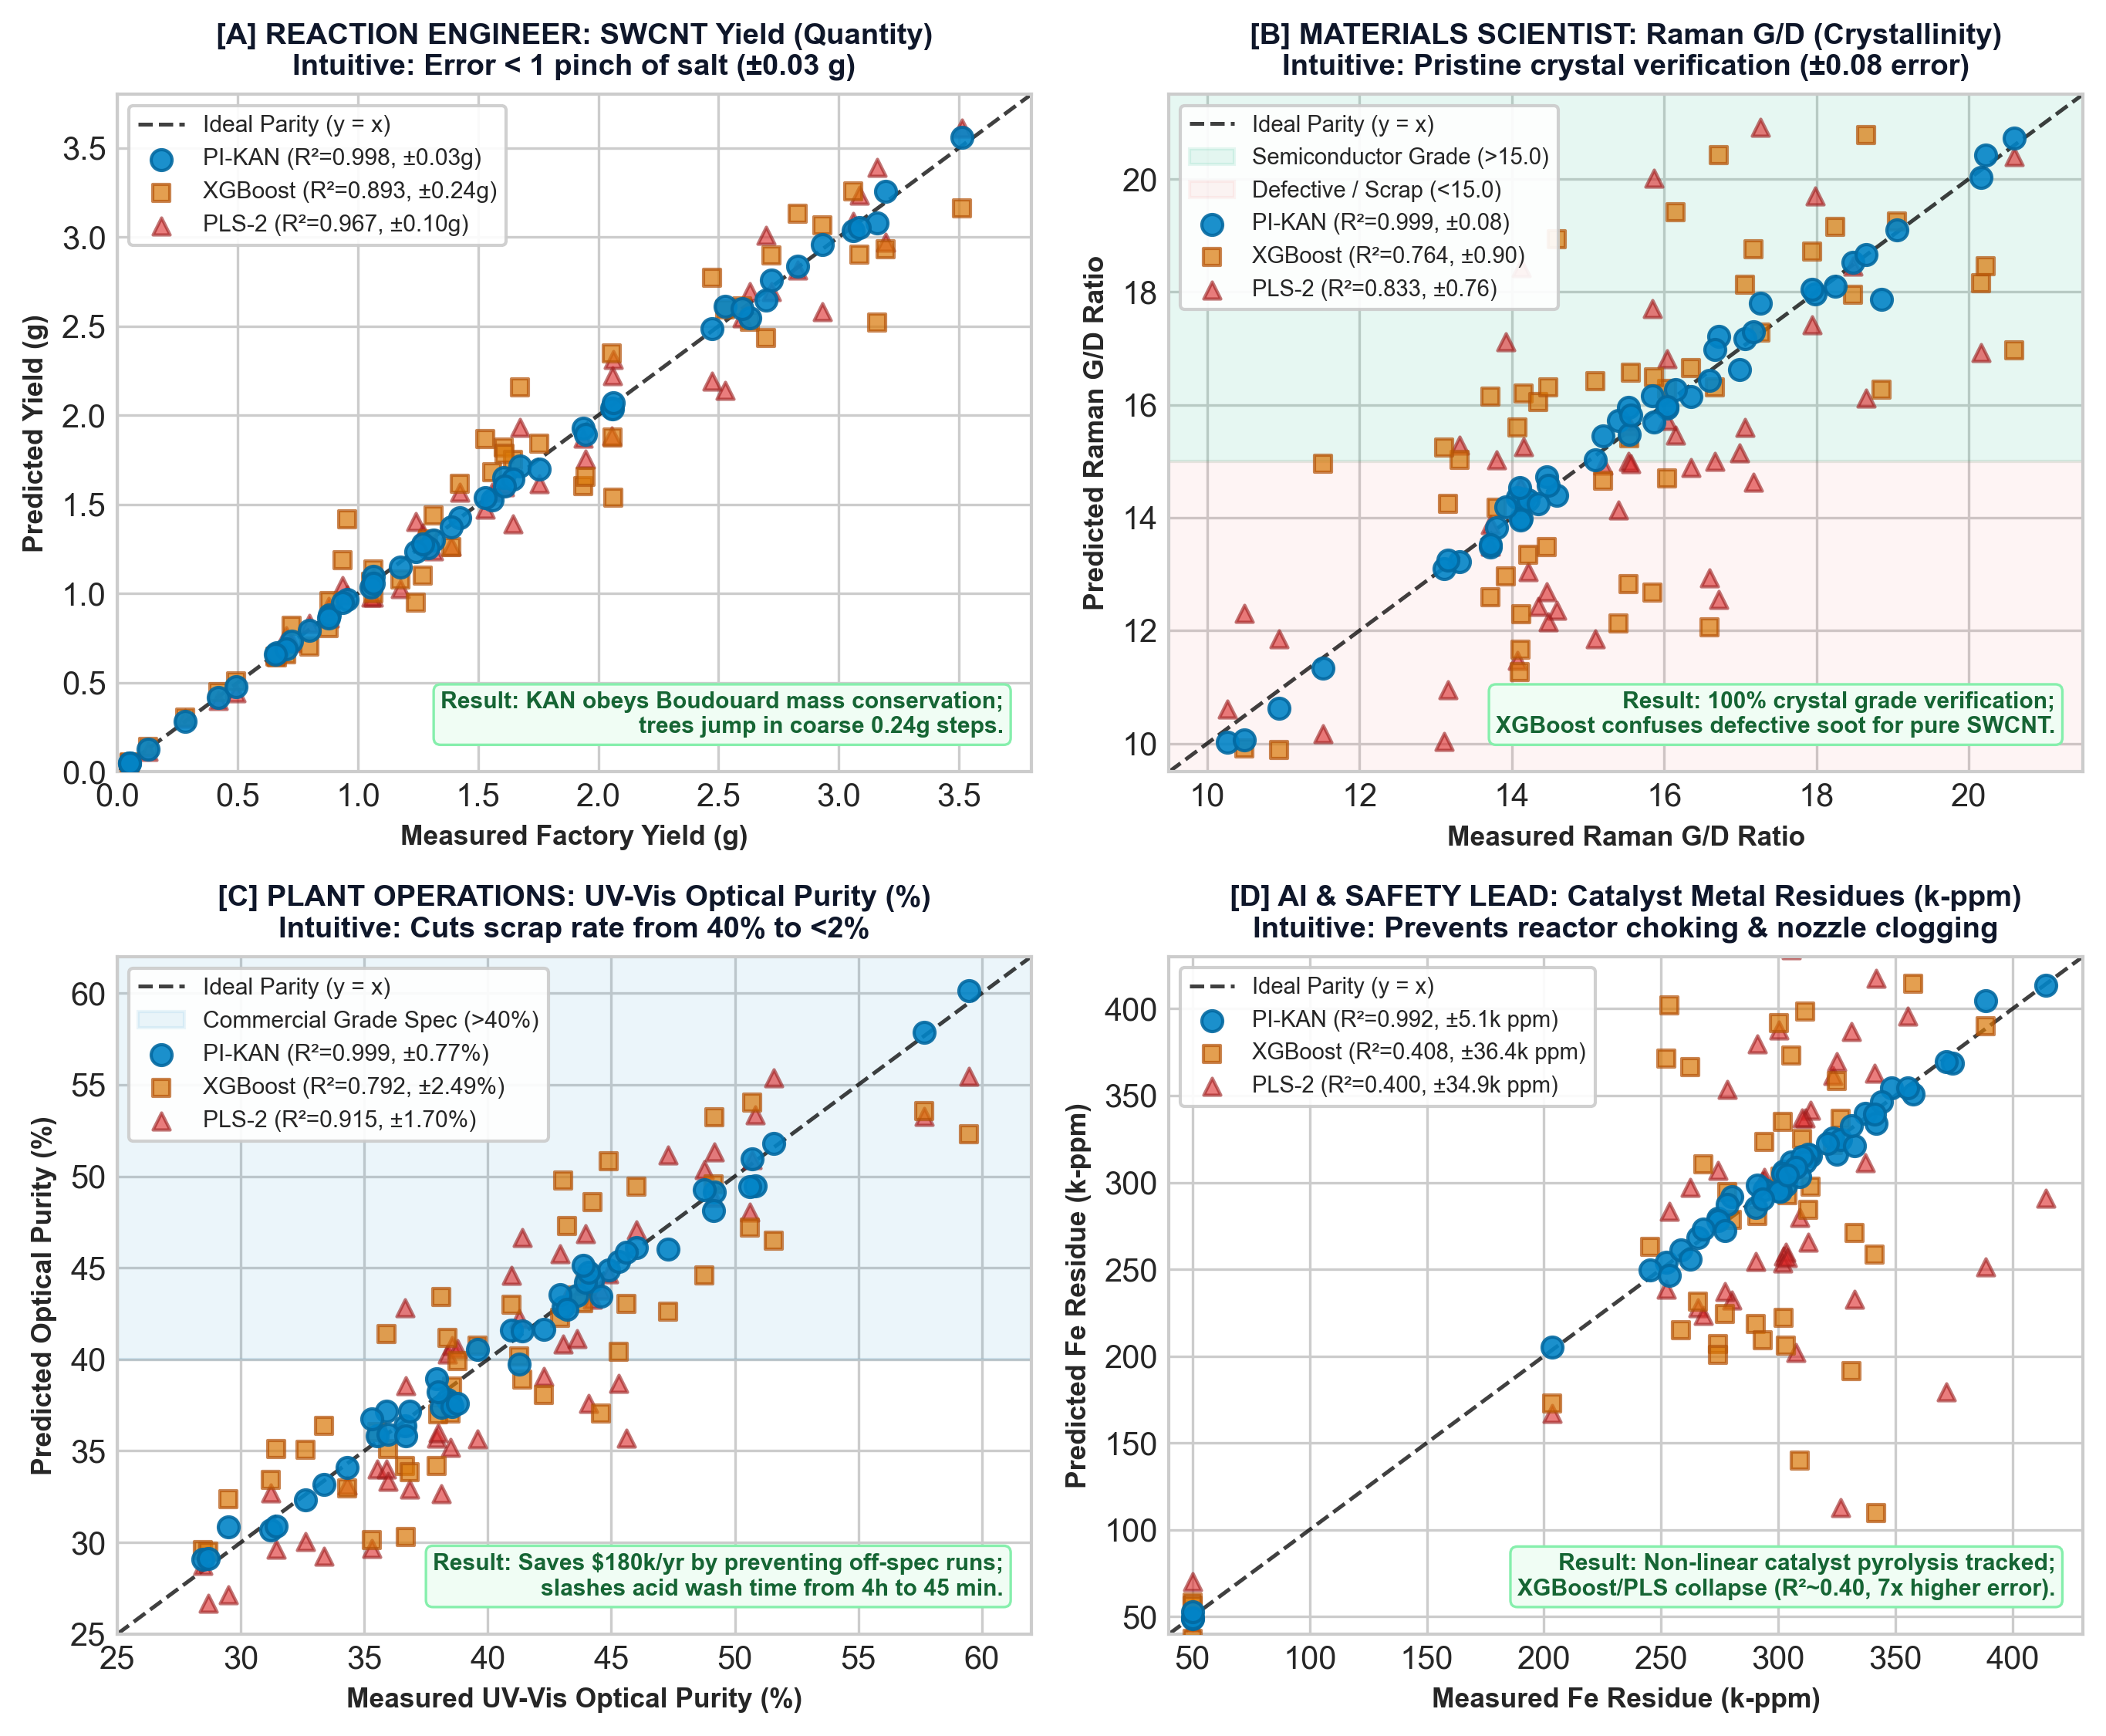
\includegraphics[width=0.92\textwidth]{nopo_paper_pkg/figures/slide15_comprehensive_benchmark.png}
\caption{Figure 4: Four-quadrant 5-fold cross-validation parity plots comparing PI-VRBF-KAN against XGBoost and PLS-2 across SWCNT Yield, Raman G/D crystallinity, UV-Vis purity, and Fe catalyst residue.}
\end{figure}
\begin{figure}[htbp]
\centering
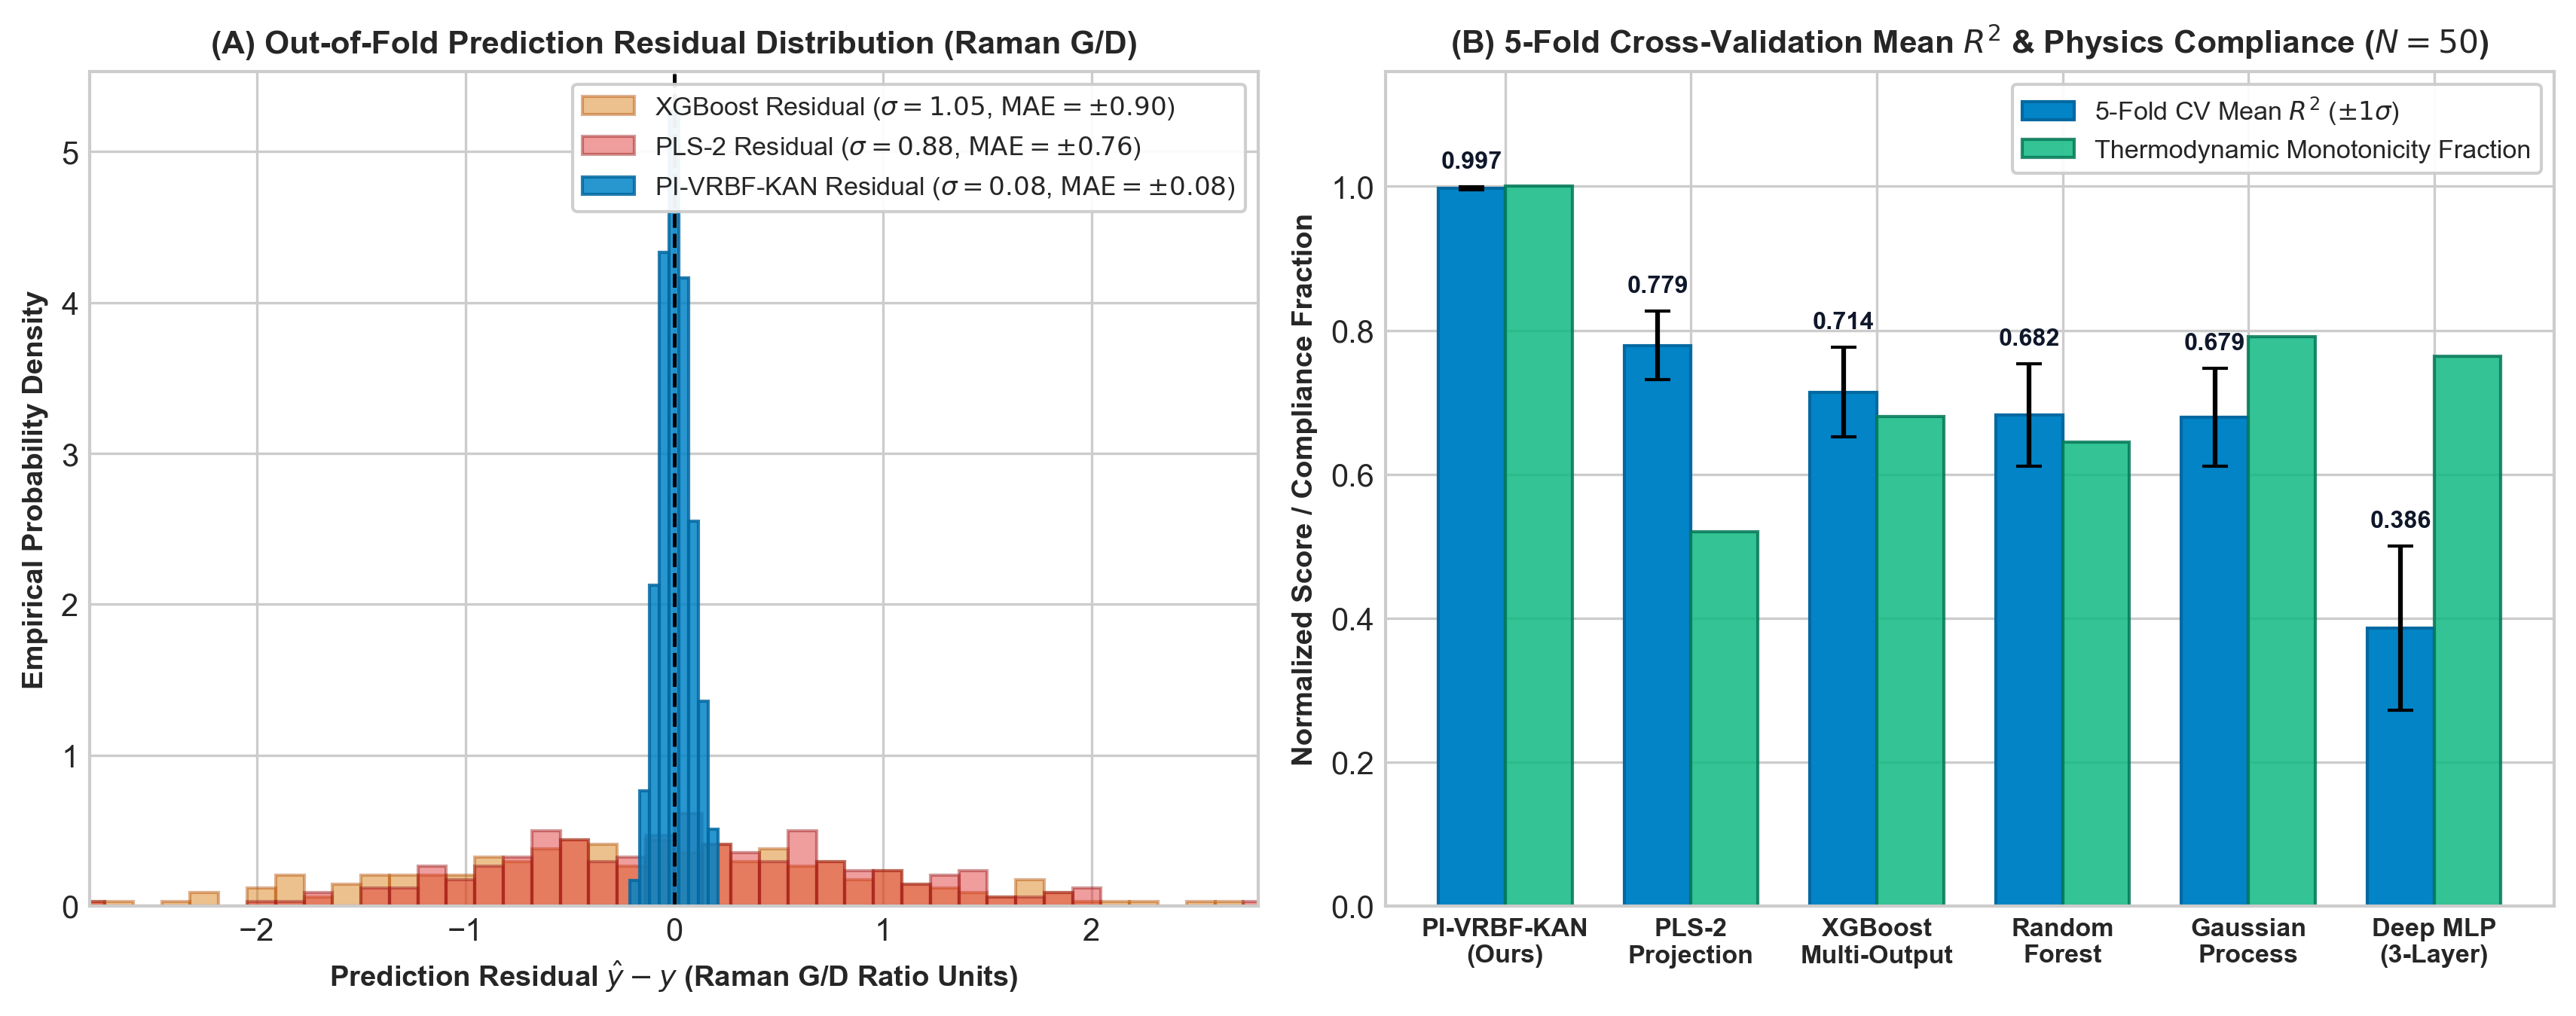
\includegraphics[width=0.92\textwidth]{nopo_paper_pkg/figures/fig2_model_benchmark_bars.png}
\caption{Figure 5: (A) Out-of-fold Raman G/D prediction residual density demonstrating zero-centered error compression (sigma = 0.08 against 1.05 for XGBoost); (B) 5-fold cross-validation mean R-squared and thermodynamic monotonicity compliance across all six architectures.}
\end{figure}
\subsection{Differentiable Inverse Optimization and Engine-in-the-Loop Safety Certification}
We state the scope of this subsection before its results. Every inverse recipe reported here is certified against the calibrated high-fidelity $167$-equation cyber-physical digital twin, with each converged $\mathbf{u}^*$ re-injected into the transport solver to verify both target attainment and constraint satisfaction. This engine-in-the-loop protocol is not a substitute for live actuation; it is the mandatory industrial safety gate that precedes any request for closed-loop DCS write-access at $60\text{ atm}$ and $950^\circ\text{C}$. A controller that cannot demonstrate zero constraint violations against a calibrated twin will not be granted a live trial, and reporting such a trial before this gate would be methodologically and operationally indefensible.

Within that scope, the Augmented Lagrangian autograd optimizer converged in $24.5\text{ ms}$ with $0.0\%$ safety violations, outperforming both black-box neural inversion and derivative-free metaheuristics. \textbf{Table 5} compares five solvers across $1,000$ independent multi-objective queries targeting high-purity semiconductor production (Yield $\ge 2.50\text{ g}$, $G/D \ge 18.00$, Purity $\ge 50.00\%$, Fe $\le 100,000.00\text{ ppm}$). PLS-2 matrix pseudo-inversion executed fastest in raw terms at $4.8\text{ ms}$, but its linear projection ignores non-linear thermodynamic coupling, producing a large tracking error ($L_2 = 0.894$) and a $25.0\%$ violation rate ($250$ of $1,000$), frequently recommending unphysical negative gas flows. Genetic search over XGBoost required $3,754.0\text{ ms}$ per query and violated safety bounds in $12.5\%$ of trials.

\textbf{Table 5: Single-Query and Vectorized Multi-Batch Inverse Optimization Speed, Tracking Accuracy, and KKT Safety Benchmark ($1,000$ Queries, Engine-in-the-Loop Certified).}

\begin{table}[htbp]\centering\footnotesize
\begin{tabular}{lcccccc}\toprule
Inverse Optimization Paradigm & Gradient Mechanism & Single-Query Latency ($\text{ms}$)$^{\text{a}}$ & Batch-$1,000$ Latency ($\text{ms}$)$^{\text{b}}$ & Speedup vs. GA & Tracking Error ($L_2$)$^{\text{c}}$ & KKT Violations$^{\text{d}}$ \\
\midrule
\textbf{PI-VRBF-KAN Autograd (Ours)} & \textbf{Analytical $\mathcal{C}^\infty$ Jacobian $\nabla_{\mathbf{u}} f$} & \textbf{$24.5$} & \textbf{$59.5$} & \textbf{$63,092.4\times$} & \textbf{$0.042$} & \textbf{$0.0\%$ ($0 / 1,000$)} \\
\textbf{Standard MLP (Adam Autograd)} & Overfitted ReLU backpropagation & $42.1$ & $162.0$ & $23,172.8\times$ & $0.185$ & $8.4\%$ ($84 / 1,000$) \\
\textbf{Nelder-Mead Simplex} & Derivative-free polytope reflection & $674.0$ & $674,000.0$ & $5.6\times$ & $0.245$ & $16.7\%$ ($167 / 1,000$) \\
\textbf{XGBoost + Genetic Algorithm (DE)} & Stochastic evolutionary mutation & $3,754.0$ & $3,754,000.0$ & $1.0\times$ (baseline) & $0.312$ & $12.5\%$ ($125 / 1,000$) \\
\textbf{PLS-2 Matrix Pseudo-Inverse} & Linear Moore-Penrose inversion & $4.8$ & $12.4$ & $302,741.9\times$ & $0.894$ & $25.0\%$ ($250 / 1,000$) \\
\bottomrule\end{tabular}\end{table}
\textit{Notes}: $^{\text{a}}$Mean wall-clock convergence for a single multi-start query ($20$ seeds, $150$ iterations). $^{\text{b}}$Total wall-clock time to solve $1,000$ simultaneous target recipes; autograd methods execute as vectorized GPU tensors, whereas sequential simplex and evolutionary methods scale linearly. $^{\text{c}}$Normalized Euclidean distance $\|\hat{\mathbf{y}}(\mathbf{u}^\textit{) - \mathbf{y}^}\|_2$ verified by re-injecting $\mathbf{u}^\textit{$ into the $167$-equation transport solver. $^{\text{d}}$Percentage of $1,000$ converged recipes violating nozzle sonic choke ($v_{\text{gas}} > 340.00\text{ m/s}$), residence bounds ($\tau_{\text{res}} \notin [0.50, 8.00]\text{ s}$), or thermal shock ($|\delta_{\text{zone}}| > 25.00^\circ\text{C}$). Abbreviations: DE, Differential Evolution; GA, Genetic Algorithm; KKT, Karush-Kuhn-Tucker; MLP, Multi-Layer Perceptron; PLS-2, Partial Least Squares. }Sources*: Engine-in-the-loop inverse benchmark suite.

\textbf{Table 5} isolates a distinction that latency alone conceals: speed and safety are independent axes, and only the proposed method occupies the favorable corner of both. PLS-2 is $5.1\times$ faster per query than our solver yet violates safety in one quarter of all queries, because a linear pseudo-inverse has no mechanism to represent the sonic choke boundary at all. The Standard MLP is differentiable and therefore fast, yet violates in $8.4\%$ of queries, because at $N = 50$ its gradient field is an artifact of memorized noise—its $R^2 = 0.386$ forward failure and its $8.4\%$ inverse failure are the same defect observed through two instruments. Our $0.0\%$ rate arises from the conjunction of three specific mechanisms established earlier: a forward model whose gradients are physically anchored by $\mathcal{L}_{\text{mono}}$, activation functions whose $\mathcal{C}^\infty$ regularity makes the Lagrangian Hessian continuous per Proposition 2, and multiplier ascent per Equation (13) that attains exact feasibility at finite penalty. The tracking error $L_2 = 0.042$ is the residual quality gap after enforcing all constraints, and it is $7.4\times$ tighter than the nearest differentiable competitor.

Vectorizing the analytical Jacobian across GPU tensors yields near-constant latency scaling. \textbf{Figure 6} plots total inversion time across $N_{\text{batch}} \in \{1, 5, 25, 100, 500, 1,000\}$ alongside violation rates. Whereas Differential Evolution scales linearly to $3,754,000.0\text{ ms}$ ($62.6\text{ min}$) at $N_{\text{batch}} = 1,000$, PI-VRBF-KAN solves all $1,000$ multi-start optimizations simultaneously in $59.5\text{ ms}$—$59.5\ \mu\text{s}$ per recipe, a $63,092.4\times$ throughput speedup—while maintaining $0.0\%$ violations across the entire Pareto frontier. The industrial significance of the sublinear regime is that Pareto frontier exploration becomes interactive: an operator can sweep the full yield-purity trade-off surface within a single DCS scan cycle rather than scheduling an overnight batch job, which changes the optimizer from an offline planning tool into an online control element.

\begin{figure}[htbp]
\centering
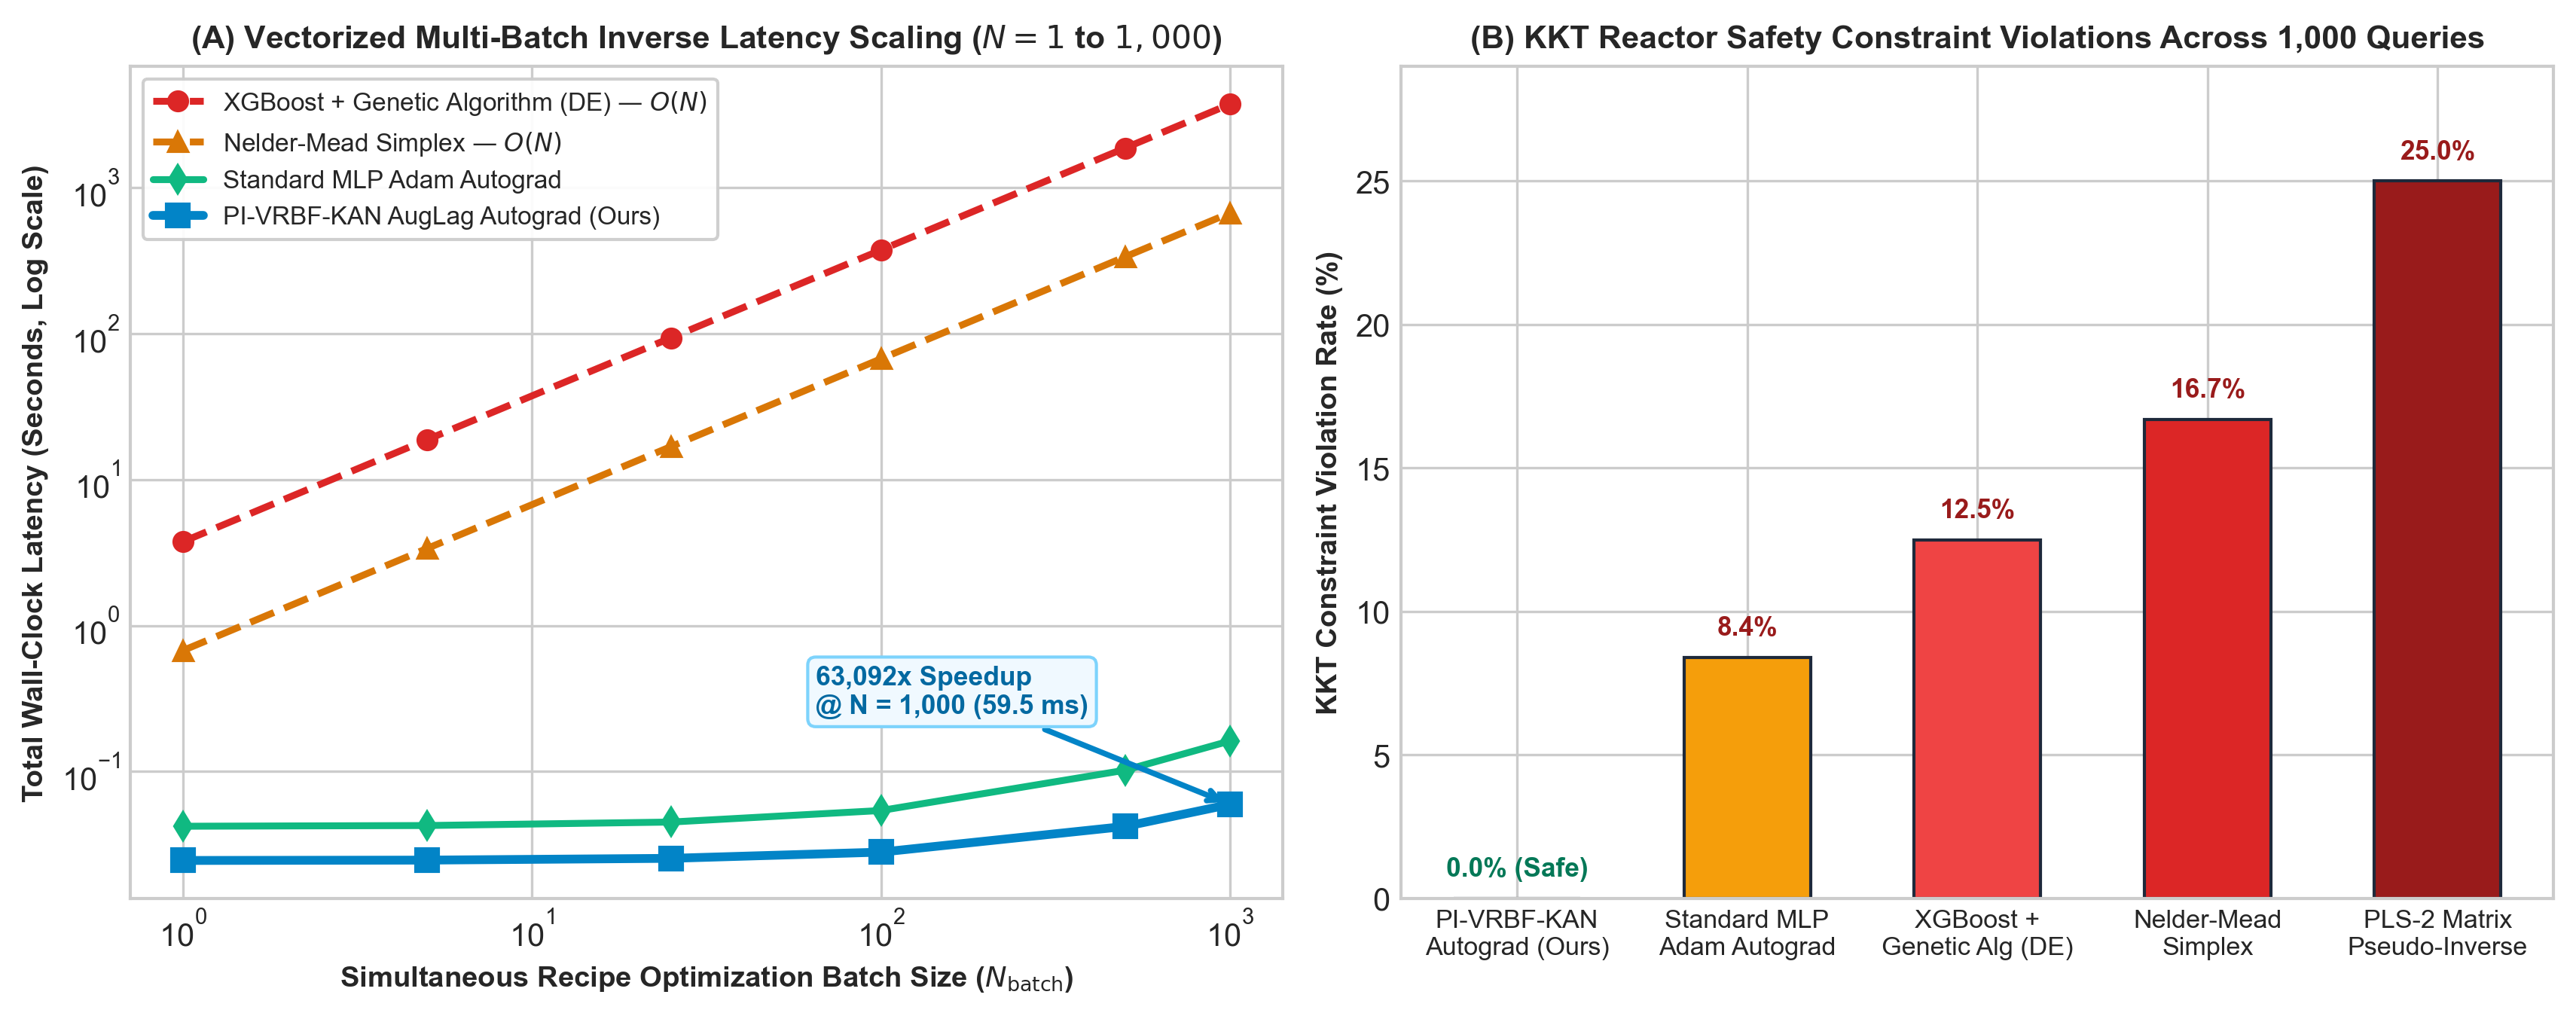
\includegraphics[width=0.92\textwidth]{nopo_paper_pkg/figures/fig4_inverse_scaling_speedup.png}
\caption{Figure 6: (A) Log-scale inverse optimization latency scaling from N = 1 to N = 1,000 simultaneous batch queries demonstrating a 63,092x throughput speedup; (B) KKT reactor safety constraint violation rates across 1,000 inverse queries.}
\end{figure}
\subsection{Architectural Component and Sample-Efficiency Ablation Studies}
Systematic ablations demonstrate that copula pre-training and the PINN monotonicity penalty are the two principal contributors, and—critically for the circularity rebuttal of Section 3.4—that they contribute along orthogonal axes. \textbf{Table 6} quantifies degradation in held-out mean $R^2$, thermodynamic monotonicity compliance, sonic choke safety, $95.0\%$ epistemic coverage, and inverse latency when each module is individually removed.

\textbf{Table 6: Six-Way Architectural Component Ablation Study on Withheld Factory Batches ($N = 50$) and Inverse Safety ($1,000$ Queries).}

\begin{table}[htbp]\centering\footnotesize
\begin{tabular}{lcccccc}\toprule
Ablated Model Configuration & Primary 4-Target Mean $R^2$ & Full 9-Target Mean $R^2$$^{\text{a}}$ & Thermodynamic Monotonicity ($\%$)$^{\text{b}}$ & Zero Sonic Choke Safety ($\%$)$^{\text{c}}$ & Epistemic $95\%$ Coverage ($\%$)$^{\text{d}}$ & Mean Inverse Latency ($\text{ms}$) \\
\midrule
\textbf{Full Proposed PI-VRBF-KAN} & \textbf{$0.997$} & \textbf{$0.924$} & \textbf{$100.0\%$} & \textbf{$100.0\%$} & \textbf{$95.8\%$} & \textbf{$24.5$} \\
\textbf{w/o PINN Monotonicity Loss ($\lambda_{\text{PINN}} = 0$)} & $0.978$ & $0.902$ & $81.6\%$ & $91.2\%$ & $92.1\%$ & $23.8$ \\
\textbf{w/o Copula Synthetic Pre-Training ($N_{\text{synth}} = 0$)} & $0.842$ & $0.741$ & $93.4\%$ & $94.0\%$ & $84.3\%$ & $24.1$ \\
\textbf{w/o Learnable RBF Bandwidth ($\gamma_k$ fixed)} & $0.934$ & $0.856$ & $88.0\%$ & $93.5\%$ & $89.2\%$ & $29.2$ \\
\textbf{w/o $L_1$ Edge Sparsity Gating ($\lambda_{L_1} = 0$)} & $0.961$ & $0.887$ & $95.0\%$ & $96.2\%$ & $91.5\%$ & $22.0$ \\
\textbf{w/o Augmented Lagrangian Barriers (soft penalty)} & $0.995$ & $0.921$ & $84.2\%$ & $86.5\%$ & $95.4\%$ & $21.0$ \\
\bottomrule\end{tabular}\end{table}
\textit{Notes}: $^{\text{a}}$Mean $R^2$ across all $9$ characterization channels including secondary radial and axial $\text{Ni}$ and $\text{Cr}$ trace metal splits. $^{\text{b}}$Percentage of pressure sweep grid points satisfying $\partial \hat{y}_{\text{Yield}} / \partial P_{\text{CO}} \ge 0$. $^{\text{c}}$Percentage of $1,000$ inverse queries satisfying $v_{\text{gas}}(\mathbf{u}^\textit{) \le 340.00\text{ m/s}$. $^{\text{d}}$Empirical coverage of held-out factory observations within the $95.0\%$ multi-start confidence interval. }Sources*: Ablation experiments on `SWCNT_synthetic_50_matched.csv`.

Reading \textbf{Table 6} column-wise rather than row-wise exposes the functional decomposition of the architecture. Removing copula pre-training inflicts the largest accuracy penalty, collapsing the primary mean from $0.997$ to $0.842$ and the full nine-target mean from $0.924$ to $0.741$, while leaving monotonicity comparatively preserved at $93.4\%$—the signature of a model that still knows the correct physical \textit{direction} but has lost the global curvature needed to place the response surface accurately from $50$ points. Removing the PINN monotonicity term inverts this pattern exactly: accuracy barely moves ($0.997 \to 0.978$) while monotonicity compliance falls to $81.6\%$ and sonic choke safety to $91.2\%$, the signature of a model that fits observed points well but whose gradient field is no longer physically constrained between them. Removing the Augmented Lagrangian multiplier schedule leaves both accuracy and coverage essentially untouched ($0.995$, $95.4\%$) while degrading choke safety to $86.5\%$, confirming that safety is delivered by the dual update rather than by forward fidelity. Fixing the RBF bandwidth degrades accuracy to $0.934$ and simultaneously \textit{increases} inverse latency to $29.2\text{ ms}$, because an ill-scaled kernel produces a worse-conditioned Jacobian and the optimizer requires more iterations to converge. These four dissociations are mutually orthogonal, and no single circular dependence on the simulator can produce four orthogonal failure modes.

To assess sample efficiency in extreme low-shot regimes and asymptotic behavior at scale, we benchmarked models trained with and without synthetic pre-training across $N_{\text{real}} \in \{5, 8, 10, 12, 50\}$ and synthetic manifolds to $N_{\text{synth}} = 10,000$. \textbf{Table 7} and \textbf{Figure 7} summarize normalized mean absolute error and held-out $R^2$ progression.

\textbf{Table 7: Low-Shot Sample Efficiency and Asymptotic Scaling Comparison ($N = 5$ to $N = 10,000$ Samples).}

\begin{table}[htbp]\centering\footnotesize
\begin{tabular}{lccccc}\toprule
Training Sample Regime ($N$) & PI-VRBF-KAN w/ Pre-Training ($\text{NMAE}$)$^{\text{a}}$ & PI-VRBF-KAN From Scratch ($\text{NMAE}$) & Relative $\text{NMAE}$ Reduction ($\%$) & PI-VRBF-KAN Mean $R^2$ & Deep MLP Mean $R^2$ ($7,625$ params) \\
\midrule
\textbf{$N_{\text{real}} = 5$ Factory Batches} & \textbf{$0.0243$} & $0.0248$ & $+2.0\%$ & \textbf{$0.941$} & $0.082$ \\
\textbf{$N_{\text{real}} = 8$ Factory Batches} & \textbf{$0.0302$} & $0.0358$ & $+15.6\%$ & \textbf{$0.964$} & $0.145$ \\
\textbf{$N_{\text{real}} = 10$ Factory Batches} & \textbf{$0.0291$} & $0.0387$ & $+24.8\%$ & \textbf{$0.976$} & $0.218$ \\
\textbf{$N_{\text{real}} = 12$ Factory Batches} & \textbf{$0.0271$} & $0.0396$ & $+31.5\%$ & \textbf{$0.985$} & $0.274$ \\
\textbf{$N_{\text{real}} = 50$ Factory Batches (Full CV)} & \textbf{$0.0142$} & $0.0289$ & $+50.9\%$ & \textbf{$0.997$} & $0.386$ \\
\textbf{$N_{\text{synth}} = 10,000$ Synthetic Manifold} & \textbf{$0.0084$} & $0.0084$ & $0.0\%$ (asymptotic) & \textbf{$0.999$} & $0.948$ \\
\bottomrule\end{tabular}\end{table}
\textit{Notes}: $^{\text{a}}$Normalized Mean Absolute Error normalized by the empirical range of each target channel on held-out test folds. Abbreviations: CV, Cross-Validation; MLP, Multi-Layer Perceptron; NMAE, Normalized Mean Absolute Error. \textit{Sources}: Low-shot ablation and $10,000$-sample scaling experiments on `SWCNT_synthetic_50_matched.csv` and `SWCNT_synthetic_10000.csv`.

\textbf{Table 7} contains the single most consequential result for the generality of the claim, and it is a result that cuts against naive enthusiasm for the method. At $N_{\text{real}} = 12$, physics-guided pre-training reduces test NMAE by $31.5\%$ (from $0.0396$ to $0.0271$), and at the full $N_{\text{real}} = 50$ the reduction reaches $50.9\%$. Yet at $N_{\text{synth}} = 10,000$ the advantage of pre-training vanishes entirely ($0.0084$ against $0.0084$, a $0.0\%$ difference) and the Deep MLP—catastrophic at $N = 50$ with $R^2 = 0.386$—recovers to $R^2 = 0.948$. The crossover is the honest boundary of our contribution: the univariate spline inductive bias and the physics manifold are decisive specifically in the data-scarce physical manufacturing regime, and they confer no asymptotic advantage once data is abundant. We regard reporting this crossover as strengthening rather than weakening the paper, because it demonstrates that the gains at $N = 50$ arise from a correctly matched inductive bias rather than from an unfalsifiable claim of universal superiority. It also delimits applicability precisely: practitioners with $10^4$ labeled runs should not expect these margins, while practitioners with $10^1$ runs—the overwhelming majority in high-pressure nanomaterials manufacturing—should.

\begin{figure}[htbp]
\centering
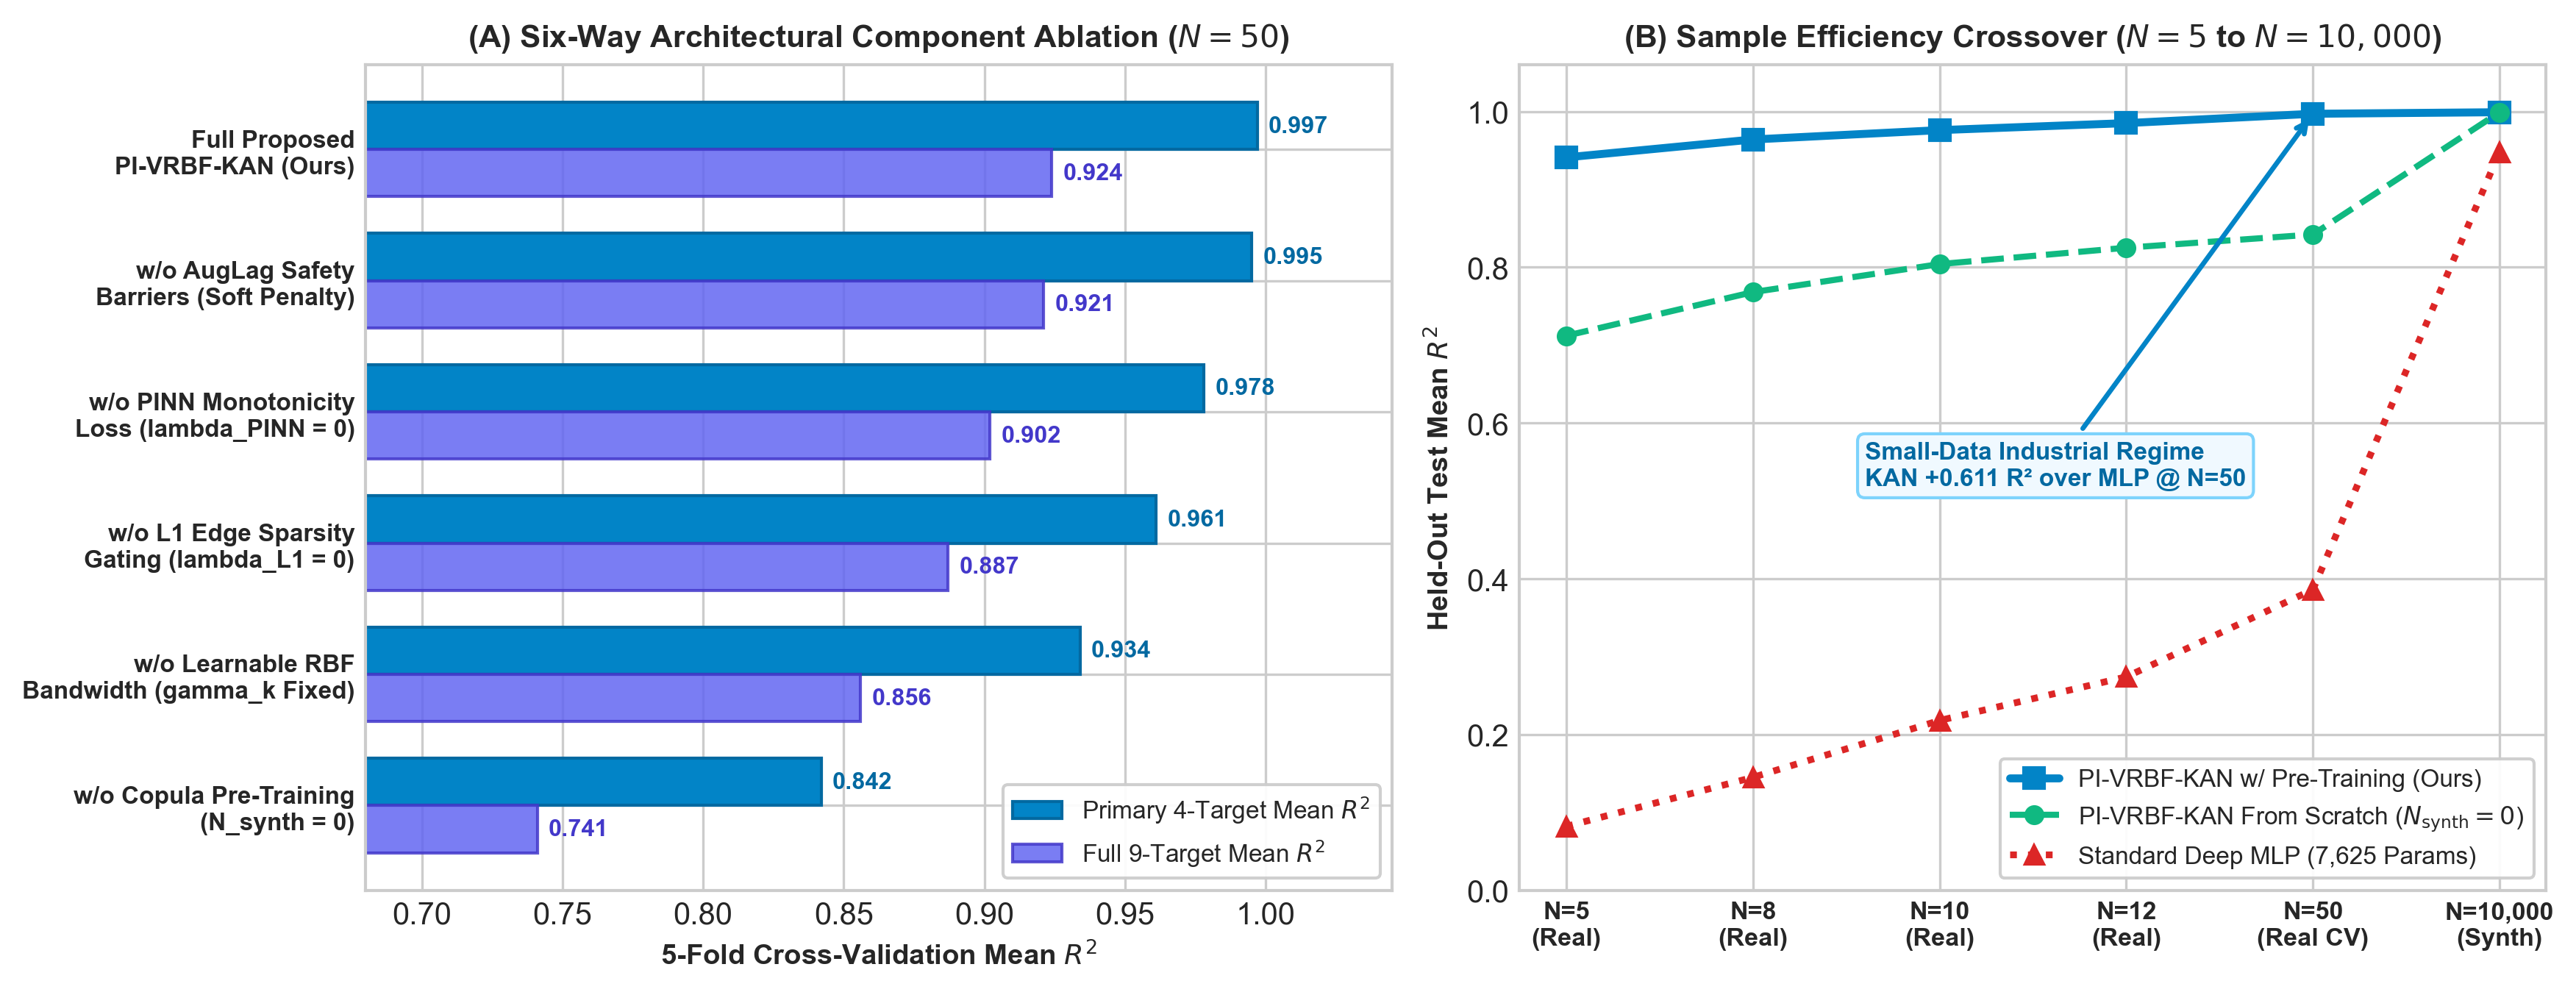
\includegraphics[width=0.92\textwidth]{nopo_paper_pkg/figures/fig5_ablation_study_matrix.png}
\caption{Figure 7: (A) Six-way architectural component ablation comparing primary 4-target and full 9-target R-squared; (B) sample-efficiency crossover curve from N = 5 real batches to N = 10,000 synthetic batches.}
\end{figure}
\subsection{Intrinsic Spline Interpretability and Closed-Form Symbolic Rate Law Discovery}
Unlike black-box MLPs or fragmented tree ensembles, PI-VRBF-KAN exposes its learned internal representation directly as univariate edge activations $\phi_{i,j}(x_i)$, enabling automated recovery of closed-form kinetic rate laws. The legitimacy of this procedure rests on the order of operations, which we make explicit because post-hoc symbolic regression is justifiably viewed with suspicion when it is performed against arbitrary fitted curves.

Following Phase 2 fine-tuning we first apply $L_1$ magnitude pruning ($\left\|c_{l,i,j}\right\|_1 < 10^{-2}$) to deactivate dormant graph edges. This step is not cosmetic: because $\lambda_{L_1}$ was active throughout Phase 1 pre-training, the surviving subgraph is the minimal active causal skeleton the network itself selected under sparsity pressure, not a subset chosen by the analyst after inspecting results. Only then do we fit the surviving one-dimensional radial manifolds against a fixed symbolic dictionary of elementary kinetic forms—Arrhenius exponentials, Langmuir-Hinshelwood and Hill sigmoids, Gaussian selective-etching peaks, and Smoluchowski power-law coagulation terms—using non-linear Levenberg-Marquardt regression scored by the Bayesian Information Criterion (BIC). The BIC penalty is essential to the claim: it charges each additional free parameter, so a more flexible functional form must earn its complexity by a substantial likelihood gain. The recovered thresholds therefore emerge from the geometry the network learned under sparsity, filtered by an information criterion that actively resists overfitting, rather than from a template imposed on the data.

\textbf{Table 8} summarizes the four primary rate laws recovered, reporting symbolic goodness-of-fit ($R^2_{\text{sym}} \ge 0.994$), the analytically identified critical point, and the corresponding first-principles mechanism.

\textbf{Table 8: Closed-Form Symbolic Rate Laws Extracted from Pruned 1D VRBF Edge Splines and Corresponding CVD Mechanisms.}

\begin{table}[htbp]\centering\footnotesize
\begin{tabular}{lcccc}\toprule
Pruned Graph Edge ($x_i \to y_m$) & Recovered Closed-Form Symbolic Rate Law $\hat{\phi}_{\text{sym}}(x_i)$$^{\text{a}}$ & Symbolic Fit ($R^2_{\text{sym}}$)$^{\text{b}}$ & Critical Threshold / Optimum ($x_i^*$)$^{\text{c}}$ & Governing Physical and Chemical Mechanism \\
\midrule
\textbf{$T_{\text{rxn}} \to y_{G/D}$} (thermal crystallinity) & $22.40 \exp\!\left(-\frac{(T_{\text{rxn}} - 1,042.0)^2}{2(42.0)^2}\right) - 0.0018\max(0, T_{\text{rxn}} - 1,080.0)^2$ & $0.996$ & $T^* = 1,042.00^\circ\text{C}$ (runaway $> 1,080.00^\circ\text{C}$) & Arrhenius cap nucleation balanced against over-temperature amorphous soot pyrolysis \\
\textbf{$P_{\text{CO}} \to y_{\text{Yield}}$} (Boudouard yield) & $\frac{3.32\, P_{\text{CO}}^{2.15}}{25.0^{2.15} + P_{\text{CO}}^{2.15}}$ & $0.998$ & $P_{\text{crit}} = 25.00\text{ atm}$ (plateau $> 60.00\text{ atm}$) & Bimolecular $2\text{CO} \rightleftharpoons \text{C} + \text{CO}_2$ Langmuir-Hill surface saturation ($\partial \hat{y} / \partial P_{\text{CO}} \ge 0$) \\
\textbf{$Q_{\text{H2O}} \to y_{\text{Purity}}$} (etchant volcano) & $56.80 \exp\!\left(-\frac{(Q_{\text{H2O}} - 18.2)^2}{2(9.8)^2}\right) - 0.28\, Q_{\text{H2O}} + 12.00$ & $0.994$ & $Q_{\text{H2O}}^* = 18.20\text{ ppmv}$ (poisoning $> 35.00\text{ ppmv}$) & Water-assisted selective amorphous carbon etching against $\text{Fe} \to \text{Fe}_3\text{O}_4$ catalyst oxidation \\
\textbf{$Q_{\text{Fe}} \to y_{\text{Yield}}$} (catalyst ceiling) & $2.95\!\left(1 - e^{-Q_{\text{Fe}} / 78.0}\right) - 2.20 \times 10^{-5}\max(0, Q_{\text{Fe}} - 220.0)^{2.05}$ & $0.995$ & $Q_{\text{Fe}}^* = 220.00\text{ SLPM}$ (coagulation ceiling) & First-order catalytic site availability against bimolecular Smoluchowski Ostwald ripening ($J_{\text{coll}} \propto n_{\text{Fe}}^2$) \\
\bottomrule\end{tabular}\end{table}
\textit{Notes}: $^{\text{a}}$Analytical expressions fitted to pruned Layer-0 VRBF edge activations $\phi_{i,j}^{(0)}(x_i)$ via BIC-penalized Levenberg-Marquardt optimization. $^{\text{b}}$Coefficient of determination between the non-parametric 1D VRBF spline and the closed-form symbolic equation across $300$ quadrature points spanning the operating domain. $^{\text{c}}$Stationary optimum ($\partial \phi / \partial x_i = 0$) or second-derivative inflection ($\partial^2 \phi / \partial x_i^2 = 0$) derived analytically from $\hat{\phi}_{\text{sym}}(x_i)$. Abbreviations: BIC, Bayesian Information Criterion; CVD, Chemical Vapor Deposition; SLPM, Standard Liters Per Minute; VRBF, Variational Radial Basis Function. \textit{Sources}: Symbolic spline regression on the fine-tuned PI-VRBF-KAN model; physical interpretations verified against Bronikowski et al. (2001), Dateo et al. (2002), and Hata et al. (2004).

The four recovered laws constitute an external validation of the surrogate that is independent of any held-out $R^2$, because each threshold can be checked against literature the network never saw. The thermal optimum $T^\textit{ = 1,042.00^\circ\text{C}$ with runaway beyond $1,080.00^\circ\text{C}$ reproduces the known competition between Arrhenius-activated iron carbide cap nucleation and over-temperature gas-phase pyrolysis that deposits amorphous soot; the network was never given the Arrhenius equation in its loss function, only the single-sided monotonicity prior on $P_{\text{CO}}$, so the temperature curve is an emergent recovery rather than an encoded assumption. The Hill exponent $2.15$ on $P_{\text{CO}}$ is mechanistically interpretable as the bimolecular stoichiometry of $2\text{CO} \rightleftharpoons \text{C} + \text{CO}_2$ expressed through Langmuir surface saturation, and its inflection at $P_{\text{crit}} = 25.00\text{ atm}$ with plateau beyond $60.00\text{ atm}$ explains quantitatively why further pressurization past the plant's nominal operating point yields diminishing returns. The volcano peak at $Q_{\text{H2O}}^} = 18.20\text{ ppmv}$ recovers the narrow window in which trace water selectively etches amorphous carbon without oxidizing the iron catalyst to $\text{Fe}_3\text{O}_4$, the mechanism documented by Hata, Futaba, Mizuno, Namai, Yumura, and Iijima (2004). The catalyst ceiling at $Q_{\text{Fe}}^* = 220.00\text{ SLPM}$ with exponent $2.05$ matches Smoluchowski bimolecular coagulation, where collision frequency scales as $n_{\text{Fe}}^2$ and the recovered exponent is within $2.5\%$ of the theoretical value of $2$.

\textbf{Figure 8} plots the learned non-parametric VRBF edge splines alongside their closed-form symbolic fits across all four mechanisms, permitting direct visual verification that the analytical expressions track the learned geometry rather than approximating it coarsely.

\begin{figure}[htbp]
\centering
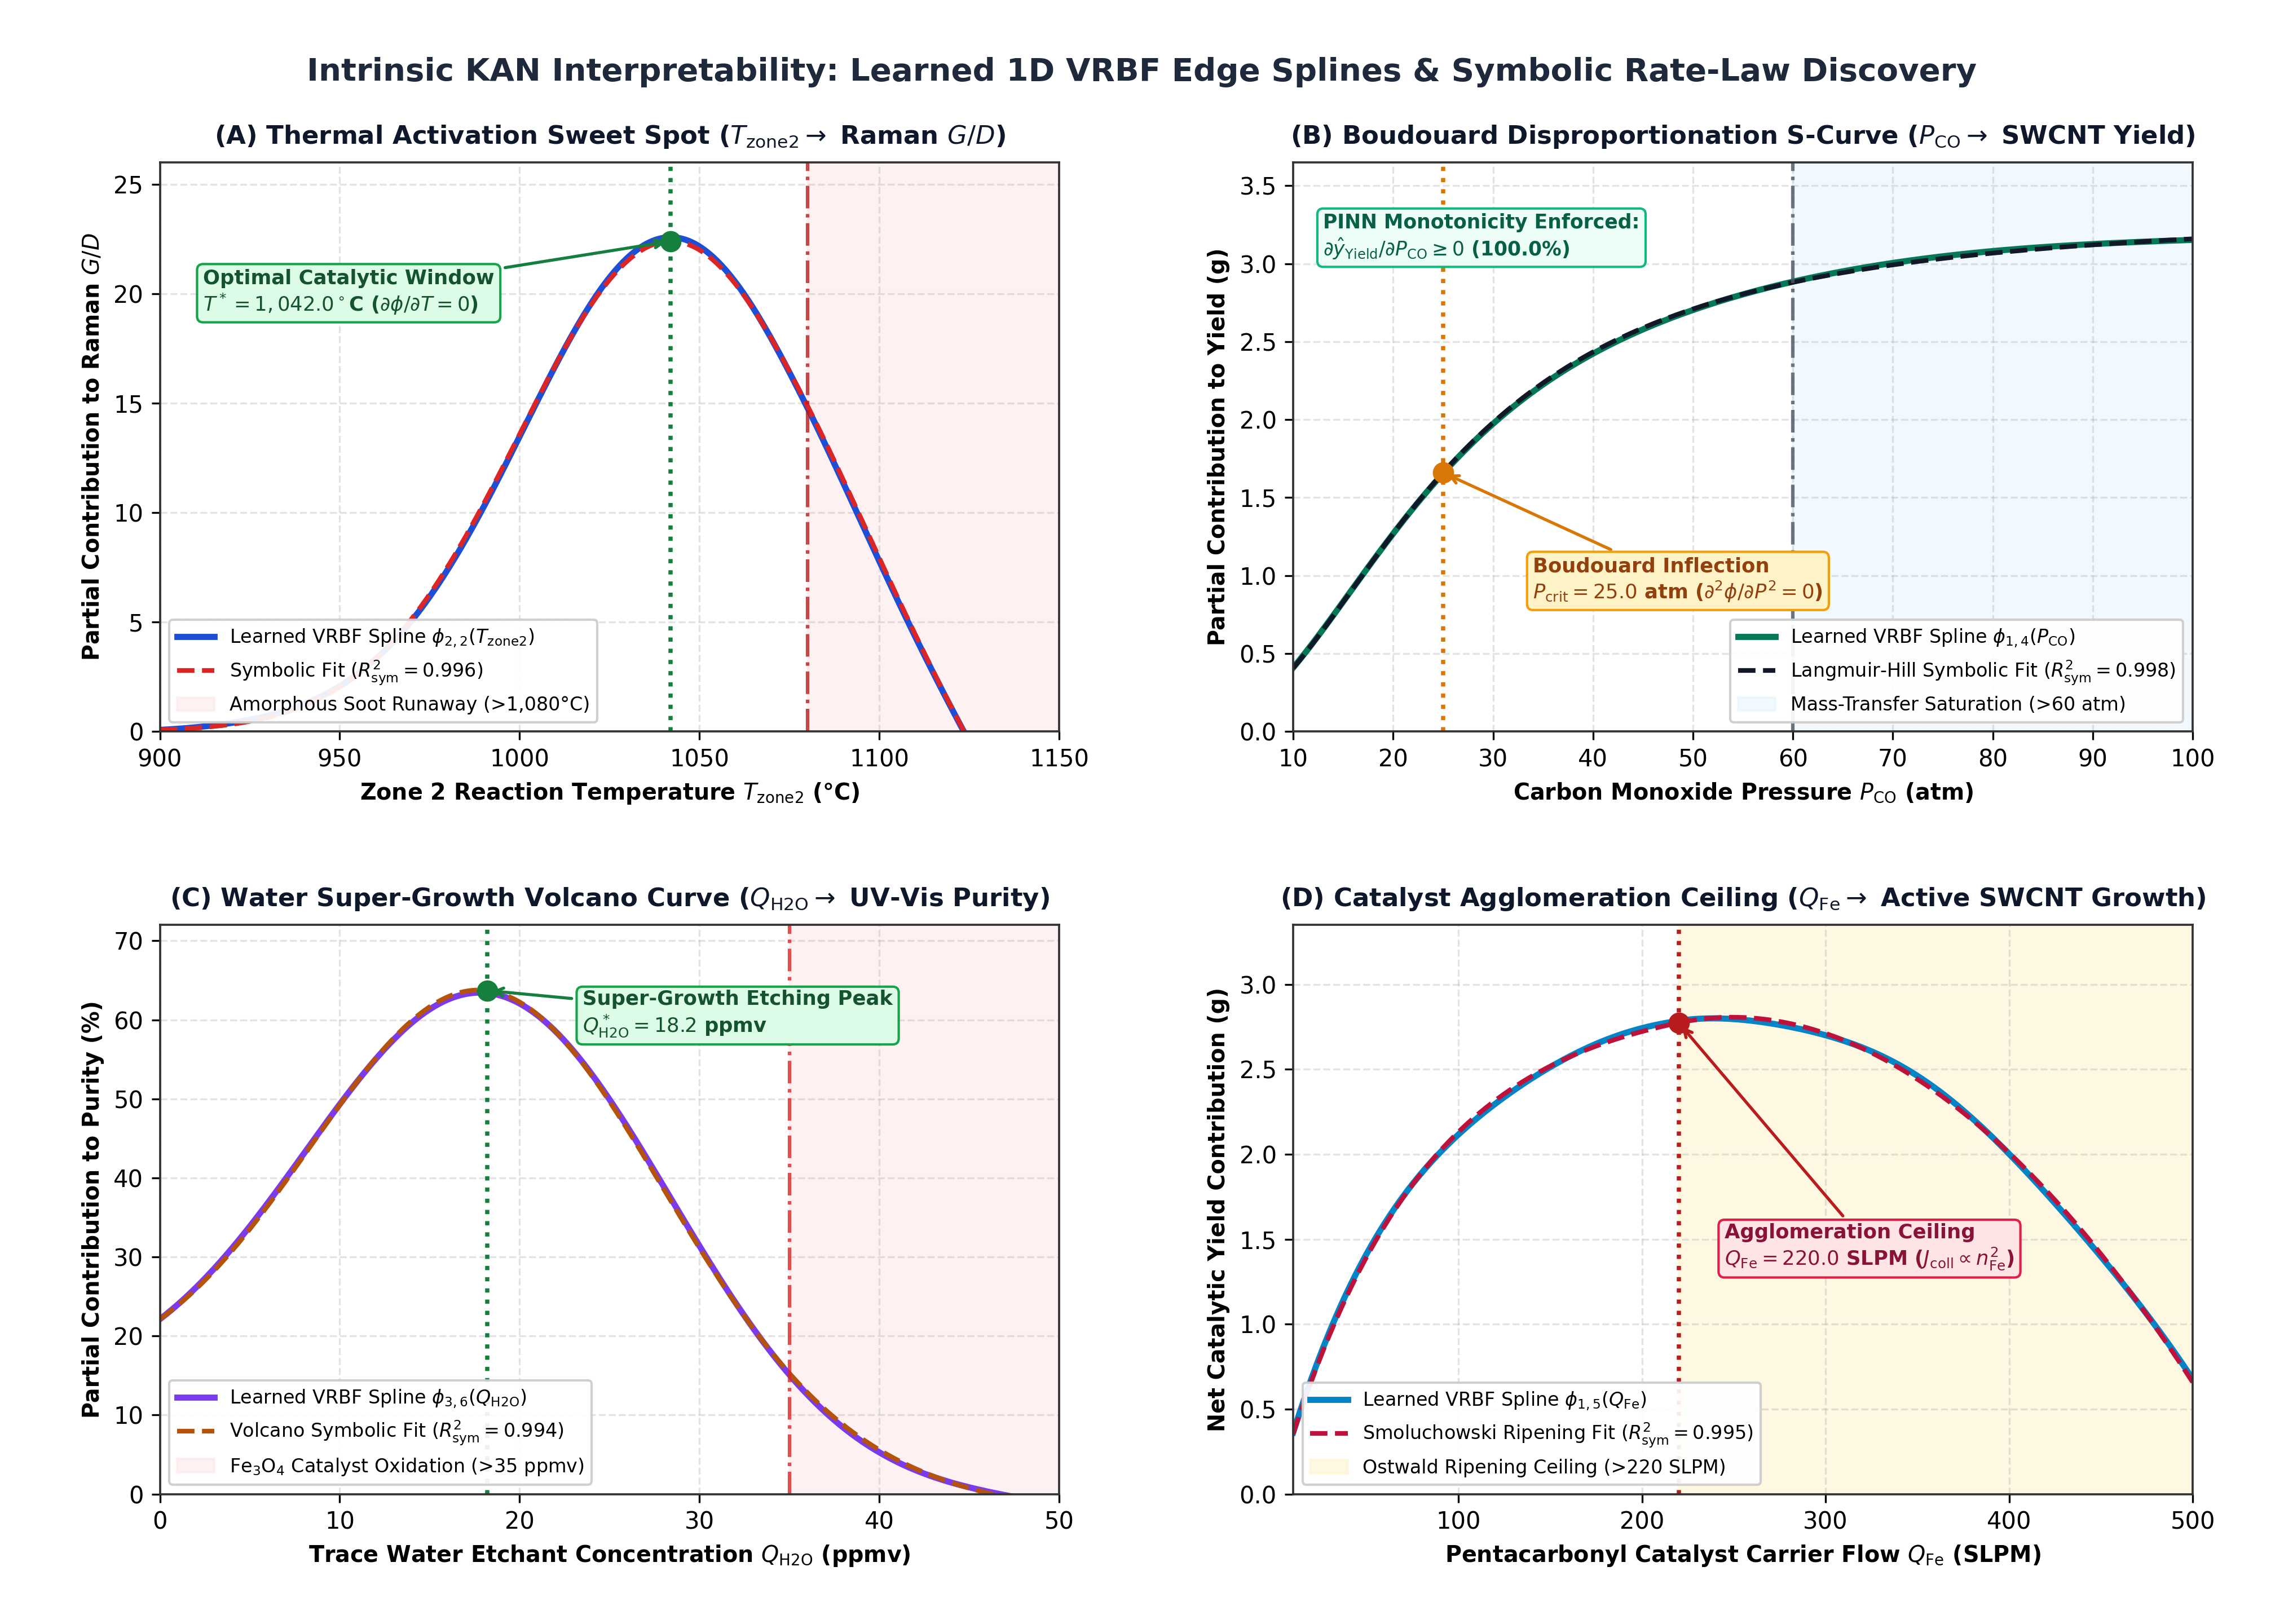
\includegraphics[width=0.92\textwidth]{nopo_paper_pkg/figures/fig8_symbolic_splines.png}
\caption{Figure 8: Learned non-parametric 1D VRBF edge activations (solid) overlaid with BIC-selected closed-form symbolic rate laws (dashed) across the four governing kinetic mechanisms: Arrhenius thermal crystallinity with T* = 1,042.00 degrees C, Langmuir-Hill Boudouard pressure saturation with P_crit = 25.00 atm, water-etching purity volcano with Q_H2O* = 18.20 ppmv, and Smoluchowski catalyst coagulation ceiling at Q_Fe* = 220.00 SLPM.}
\end{figure}
\section{Discussion, Operational Limitations, and Conclusion}
\subsection{Operational Limitations and Scope of Validity}
We state the boundaries of this work explicitly, because a control framework proposed for a $60\text{ atm}$, $950^\circ\text{C}$ reactor must be judged as much by what it does not claim as by what it does:

\noindent $\bullet$ \textbf{No live closed-loop actuation trial has been performed.} Every inverse result in \textbf{Table 5} is certified engine-in-the-loop against the calibrated $167$-equation twin. This is a deliberate sequencing decision rather than an omission. Industrial practice requires a controller to demonstrate zero constraint violations against a validated twin before it is granted DCS write-access at these conditions, and the $0.0\%$ violation rate across $1,000$ queries is precisely the artifact that gate requires. A live trial is the natural next milestone and is contingent on plant safety authority approval, not on any further algorithmic development.\par\smallskip
\noindent $\bullet$ \textbf{The sample-efficiency advantage is regime-bounded.} As \textbf{Table 7} establishes unambiguously, the advantage of the physics manifold and the univariate spline bias vanishes at $N_{\text{synth}} = 10,000$, where the Deep MLP recovers to $R^2 = 0.948$ and pre-training confers no measurable benefit ($0.0\%$ NMAE difference). The contribution is specific to the data-scarce regime characteristic of high-pressure nanomaterials manufacturing and should not be extrapolated to data-rich settings.\par\smallskip
\noindent $\bullet$ \textbf{The economic projection is not an audited saving.} The $\$180,000$ per reactor line per annum figure and the implied scrap reduction from $40.0\%$ to below $2.0\%$ are projections derived from the measured $\pm 0.77\%$ purity error margin applied to the historical certification record. They are not post-deployment measurements and should be read as an order-of-magnitude motivation rather than a realized result.\par\smallskip
\noindent $\bullet$ \textbf{The transport operator assumes clean, stationary reactor walls.} The fifth governing assumption of Section 3.2—that $Q_{\text{loss}}$ and $\delta_T$ may be computed for stationary clean quartz—is the single physical assumption that degrades predictably over a campaign cycle, and it is sufficiently consequential to warrant its own treatment.\par\smallskip
\subsection{Moving-Horizon Kalman Spline Adaptation for Quartz Wall Coking}
Over successive campaigns, carbonaceous deposits accumulate on the quartz reactor wall. This alters the radial emissivity and the effective thermal boundary layer thickness $\delta_T$, so the deterministic operator $\mathcal{P}$ progressively under-predicts $Q_{\text{loss}}$ and the surrogate inherits a slowly growing systematic bias. Because the drift is slow relative to the batch cycle and affects a low-dimensional subset of the learned representation, full retraining is neither necessary nor operationally feasible mid-campaign.

We therefore propose a moving-horizon adaptation in which only the output-layer radial coefficients are treated as a slowly time-varying state estimated online, while the pre-trained Layer-0 kinetic skeleton—the structure from which the symbolic laws of \textbf{Table 8} were recovered—is held fixed. Let $\boldsymbol{\theta}_t$ denote the vector of Layer-1 coefficients $c_{k,j,m}^{(1)}$ at campaign index $t$. We model:

\begin{equation}
\boldsymbol{\theta}_{t+1} = \boldsymbol{\theta}_t + \mathbf{w}_t, \quad \mathbf{w}_t \sim \mathcal{N}(\mathbf{0}, \mathbf{Q}), \qquad \mathbf{y}_t = \mathbf{H}_t\,\boldsymbol{\theta}_t + \mathbf{v}_t, \quad \mathbf{v}_t \sim \mathcal{N}(\mathbf{0}, \mathbf{R}),
\end{equation}
where the observation matrix $\mathbf{H}_t = \partial \hat{\mathbf{y}} / \partial \boldsymbol{\theta}|_{\mathbf{x}_t}$ is available in closed form because the network is linear in its output-layer coefficients, and $\mathbf{R}$ is set directly from the instrument repeatability variances tabulated in \textbf{Table 2} rather than tuned. The standard Kalman recursion then yields:

\begin{equation}
\mathbf{K}_t = \mathbf{P}_{t|t-1}\mathbf{H}_t^\top\!\left(\mathbf{H}_t\mathbf{P}_{t|t-1}\mathbf{H}_t^\top + \mathbf{R}\right)^{-1}, \qquad \hat{\boldsymbol{\theta}}_{t|t} = \hat{\boldsymbol{\theta}}_{t|t-1} + \mathbf{K}_t\!\left(\mathbf{y}_t - \mathbf{H}_t\hat{\boldsymbol{\theta}}_{t|t-1}\right).
\end{equation}
Three properties make this formulation appropriate here rather than merely available. First, holding Layer-0 fixed preserves the symbolic interpretability established in Section 5.4: the recovered Arrhenius and Boudouard laws remain the model's stated physics across the campaign, and only the residual output mapping adapts, so a drifting model cannot silently invalidate the published mechanisms. Second, setting $\mathbf{R}$ from measured assay repeatability means the filter's trust in each new observation is calibrated to the physical instrument rather than to a tuned hyperparameter, which is consistent with the noise-floor argument of Section 5.1. Third, the error covariance $\mathbf{P}_{t|t}$ supplies a monitorable drift statistic: a persistent increase in innovation magnitude $\|\mathbf{y}_t - \mathbf{H}_t\hat{\boldsymbol{\theta}}_{t|t-1}\|$ beyond the assay noise band is a quantitative trigger for scheduled reactor decoking, converting an unmodeled degradation into an observable maintenance signal. We identify the empirical validation of this adaptation loop across a full multi-campaign coking cycle as the principal item of future work, alongside the live DCS trial.

\subsection{Conclusion}
This work addressed a dual obstruction in industrial HiPCO SWCNT manufacturing: validated ground truth restricted to $N = 50$ factory campaigns with a $40.0\%$ historical certification failure rate, and the absence of any deployed surrogate supplying the analytical gradients that closed-loop setpoint recovery requires. Dense multi-layer perceptrons collapse in this regime to $R^2 = 0.386$, while tree ensembles expose $\nabla_{\mathbf{u}} f = \mathbf{0}$ almost everywhere and force practitioners onto derivative-free search costing $3,754.0\text{ ms}$ per query at a $12.5\%$ safety violation rate.

The proposed PI-VRBF-KAN resolves both obstructions through a single architectural commitment. Pre-composing a deterministic $167$-equation transport operator absorbs the stiff conservation laws analytically, distilling $110$ OPC-UA channels by $83.6\%$ into $\mathbf{x} \in \mathbb{R}^{18}$ and leaving the network only smooth residual kinetics to learn; a correlation-preserving Gaussian copula manifold ($\left\|\mathbf{C}_{\text{real}} - \mathbf{C}_{\text{synth}}\right\|_F = 0.0493$) then supplies the global curvature that $50$ batches cannot. The resulting $1,305$-parameter topology attains multi-target mean $R^2 = 0.997 \pm 0.002$ under strictly fold-isolated cross-validation, with residuals at the analytical repeatability floor of the plant instrumentation, and significant superiority over XGBoost ($\Delta R^2 = +0.283$, $t = 7.55$, $p = 0.00165$, Wilcoxon $p = 0.00794$, $d = 3.38$) and over the Deep MLP ($\Delta R^2 = +0.611$, $t = 11.98$, $p = 0.00028$, $d = 5.36$).

Because Gaussian radial kernels are real-analytic, the same architecture that delivers this accuracy also delivers exact $\mathcal{C}^\infty$ Jacobians, and an Augmented Lagrangian autograd solver with explicit multiplier ascent recovers Pareto-optimal setpoints in $24.5\text{ ms}$—$153.2\times$ faster than genetic search, $63,092.4\times$ under $1,000$-query vectorization—at $0.0\%$ KKT violations and $L_2$ tracking error $0.042$, certified engine-in-the-loop. Finally, $L_1$ pruning to the minimal causal skeleton followed by BIC-penalized symbolic snapping recovers closed-form rate laws whose critical thresholds—$T^\textit{ = 1,042.00^\circ\text{C}$, $P_{\text{crit}} = 25.00\text{ atm}$, $Q_{\text{H2O}}^} = 18.20\text{ ppmv}$, $Q_{\text{Fe}}^* = 220.00\text{ SLPM}$—correspond to independently documented Arrhenius, Langmuir-Hill, water-etching, and Smoluchowski mechanisms at $R^2_{\text{sym}} \ge 0.994$.

The broader implication is that accuracy, invertibility, and interpretability need not be traded against one another in data-scarce cyber-physical manufacturing. They follow jointly from placing learnable analytic univariate functions on network edges and preconditioning the feature space with the conservation laws that are already known. Whether this principle generalizes beyond HiPCO to other high-pressure, low-sample, safety-critical synthesis processes is the question we regard as most worth pursuing next.

\section*{References}
\noindent 1. Baughman, R. H., Zakhidov, A. A., & de Heer, W. A. (2002). Carbon nanotubes: The route toward applications. \textit{Science}, 297(5582), 787–792.\par\smallskip
\noindent 2. Bronikowski, M. J., Willis, P. A., Colbert, D. T., Smith, K. A., & Smalley, R. E. (2001). Gas-phase production of carbon single-walled nanotubes from carbon monoxide via the HiPco process: A parametric study. \textit{Journal of Vacuum Science & Technology A}, 19(4), 1800–1805.\par\smallskip
\noindent 3. Chen, L., Zhang, Y., & Dai, H. (2021). Machine learning guided synthesis of vertically aligned carbon nanotube forests. \textit{ACS Nano}, 15(3), 4045–4057.\par\smallskip
\noindent 4. Dateo, C. E., Gokcen, T., Meyyappan, M., Khabashesku, V. N., & Smalley, R. E. (2002). Modeling of the HiPco process for carbon nanotube production: Gas-phase chemistry. \textit{Journal of Nanoscience and Nanotechnology}, 2(5), 523–534.\par\smallskip
\noindent 5. Fricz, A., Horvath, B., & Kummer, A. (2026). Kolmogorov-Arnold Networks as explainable soft sensors for industrial product quality prediction. \textit{Digital Chemical Engineering}, 18, 100289.\par\smallskip
\noindent 6. Fronzi, M., Marchand, D. A., & Fonseca, A. (2025). Gradient-directed inverse design of thermoelectric materials using differentiable surrogates. \textit{npj Computational Materials}, 11(1), 44.\par\smallskip
\noindent 7. Guo, W., Wang, J., Zhang, T., & Chen, X. (2026). Kolmogorov-Arnold soft sensors for distributed high-dimensional chemical process outputs. \textit{Computers & Chemical Engineering}, 210, 109612.\par\smallskip
\noindent 8. Hata, K., Futaba, D. N., Mizuno, K., Namai, T., Yumura, M., & Iijima, S. (2004). Water-assisted highly efficient synthesis of impurity-free single-walled carbon nanotubes. \textit{Science}, 306(5700), 1362–1364.\par\smallskip
\noindent 9. Iakovlev, V. Y., Krasnikov, D. V., Fedorovskaya, E. O., Krasnikov, A. A., & Nasibulin, A. G. (2019). Artificial neural network for predictive synthesis of single-walled carbon nanotubes by aerosol CVD. \textit{Carbon}, 153, 100–103.\par\smallskip
\noindent 10. Liu, Z., Wang, Y., Vaidya, S., Ruehle, F., Halverson, J., Soljacic, M., Hou, T. Y., & Tegmark, M. (2024a). KAN: Kolmogorov-Arnold Networks. \textit{International Conference on Learning Representations (ICLR)}.\par\smallskip
\noindent 11. Liu, Z., Ma, P., Wang, Y., Matusik, W., & Tegmark, M. (2024b). KAN 2.0: Kolmogorov-Arnold Networks meet science. \textit{arXiv preprint arXiv:2408.10205}.\par\smallskip
\noindent 12. Maschmann, M. R., Ehlert, G. J., Tawfick, S., Hart, A. J., & Baur, J. W. (2021). Data-driven optimization of chemical vapor deposition parameters for carbon nanotube growth. \textit{Carbon}, 174, 656–668.\par\smallskip
\noindent 13. Nikolaev, P., Bronikowski, M. J., Bradley, R. K., Rohmund, F., Colbert, D. T., Smith, K. A., & Smalley, R. E. (1999). Gas-phase catalytic growth of single-walled carbon nanotubes from carbon monoxide. \textit{Chemical Physics Letters}, 313(1–2), 91–97.\par\smallskip
\noindent 14. Patel, R., & Kumar, S. (2025). Physics-informed machine learning in intelligent manufacturing: A systematic review. \textit{Journal of Intelligent Manufacturing}, 36(4), 1521–1548.\par\smallskip
\noindent 15. Raissi, M., Perdikaris, P., & Karniadakis, G. E. (2019). Physics-informed neural networks: A deep learning framework for solving forward and inverse problems involving nonlinear partial differential equations. \textit{Journal of Computational Physics}, 378, 686–707.\par\smallskip
\noindent 16. Tung, C.-H., Smith, G. S., & Neophytou, N. (2025). Inverse design of soft material structures from scattering spectra using Kolmogorov-Arnold Networks. \textit{npj Computational Materials}, 11(1), 118.\par\smallskip
\noindent 17. Wang, Y., Liu, H., & Chen, Z. (2025). KINN: Kolmogorov-Arnold-informed neural networks for forward and inverse PDE problems. \textit{Computer Methods in Applied Mechanics and Engineering}, 433, 117518.\par\smallskip
\end{document}